\documentclass[twoside]{book}

% Packages required by doxygen
\usepackage{calc}
\usepackage{doxygen}
\usepackage{graphicx}
\usepackage[utf8]{inputenc}
\usepackage{makeidx}
\usepackage{multicol}
\usepackage{multirow}
\usepackage{textcomp}
\usepackage[table]{xcolor}

% Font selection
\usepackage[T1]{fontenc}
\usepackage{mathptmx}
\usepackage[scaled=.90]{helvet}
\usepackage{courier}
\usepackage{amssymb}
\usepackage{sectsty}
\renewcommand{\familydefault}{\sfdefault}
\allsectionsfont{%
  \fontseries{bc}\selectfont%
  \color{darkgray}%
}
\renewcommand{\DoxyLabelFont}{%
  \fontseries{bc}\selectfont%
  \color{darkgray}%
}

% Page & text layout
\usepackage{geometry}
\geometry{%
  a4paper,%
  top=2.5cm,%
  bottom=2.5cm,%
  left=2.5cm,%
  right=2.5cm%
}
\tolerance=750
\hfuzz=15pt
\hbadness=750
\setlength{\emergencystretch}{15pt}
\setlength{\parindent}{0cm}
\setlength{\parskip}{0.2cm}
\makeatletter
\renewcommand{\paragraph}{%
  \@startsection{paragraph}{4}{0ex}{-1.0ex}{1.0ex}{%
    \normalfont\normalsize\bfseries\SS@parafont%
  }%
}
\renewcommand{\subparagraph}{%
  \@startsection{subparagraph}{5}{0ex}{-1.0ex}{1.0ex}{%
    \normalfont\normalsize\bfseries\SS@subparafont%
  }%
}
\makeatother

% Headers & footers
\usepackage{fancyhdr}
\pagestyle{fancyplain}
\fancyhead[LE]{\fancyplain{}{\bfseries\thepage}}
\fancyhead[CE]{\fancyplain{}{}}
\fancyhead[RE]{\fancyplain{}{\bfseries\leftmark}}
\fancyhead[LO]{\fancyplain{}{\bfseries\rightmark}}
\fancyhead[CO]{\fancyplain{}{}}
\fancyhead[RO]{\fancyplain{}{\bfseries\thepage}}
\fancyfoot[LE]{\fancyplain{}{}}
\fancyfoot[CE]{\fancyplain{}{}}
\fancyfoot[RE]{\fancyplain{}{\bfseries\scriptsize Generated on Thu Nov 27 2014 13\-:10\-:25 for Expen\-Share by Doxygen }}
\fancyfoot[LO]{\fancyplain{}{\bfseries\scriptsize Generated on Thu Nov 27 2014 13\-:10\-:25 for Expen\-Share by Doxygen }}
\fancyfoot[CO]{\fancyplain{}{}}
\fancyfoot[RO]{\fancyplain{}{}}
\renewcommand{\footrulewidth}{0.4pt}
\renewcommand{\chaptermark}[1]{%
  \markboth{#1}{}%
}
\renewcommand{\sectionmark}[1]{%
  \markright{\thesection\ #1}%
}

% Indices & bibliography
\usepackage{natbib}
\usepackage[titles]{tocloft}
\setcounter{tocdepth}{3}
\setcounter{secnumdepth}{5}
\makeindex

% Hyperlinks (required, but should be loaded last)
\usepackage{ifpdf}
\ifpdf
  \usepackage[pdftex,pagebackref=true]{hyperref}
\else
  \usepackage[ps2pdf,pagebackref=true]{hyperref}
\fi
\hypersetup{%
  colorlinks=true,%
  linkcolor=blue,%
  citecolor=blue,%
  unicode%
}

% Custom commands
\newcommand{\clearemptydoublepage}{%
  \newpage{\pagestyle{empty}\cleardoublepage}%
}


%===== C O N T E N T S =====

\begin{document}

% Titlepage & ToC
\hypersetup{pageanchor=false}
\pagenumbering{roman}
\begin{titlepage}
\vspace*{7cm}
\begin{center}%
{\Large Expen\-Share }\\
\vspace*{1cm}
{\large Generated by Doxygen 1.8.6}\\
\vspace*{0.5cm}
{\small Thu Nov 27 2014 13:10:25}\\
\end{center}
\end{titlepage}
\clearemptydoublepage
\tableofcontents
\clearemptydoublepage
\pagenumbering{arabic}
\hypersetup{pageanchor=true}

%--- Begin generated contents ---
\chapter{Main Page}
\label{index}\hypertarget{index}{}\begin{DoxyAuthor}{Authors}
Taylor Andrews, Ian Char, Brennan Mc\-Connell 
\end{DoxyAuthor}
\begin{DoxyDate}{Date}
11/26/2014
\end{DoxyDate}
Expen\-Share is an online application designed to help people split costs and share expenses. You can now create one or more group(s) with your friends and log your transactions, then let Expen\-Share do the work and calculate how much each group member owes each other. This application can be used for roommates to split living expenses, friends to split travel costs, or any other necessary use! 
\chapter{Namespace Index}
\section{Packages}
Here are the packages with brief descriptions (if available)\-:\begin{DoxyCompactList}
\item\contentsline{section}{\hyperlink{namespaceforms}{forms} }{\pageref{namespaceforms}}{}
\item\contentsline{section}{\hyperlink{namespacemodels}{models} }{\pageref{namespacemodels}}{}
\item\contentsline{section}{\hyperlink{namespaceurls}{urls} }{\pageref{namespaceurls}}{}
\item\contentsline{section}{\hyperlink{namespaceviews}{views} }{\pageref{namespaceviews}}{}
\end{DoxyCompactList}

\chapter{Hierarchical Index}
\section{Class Hierarchy}
This inheritance list is sorted roughly, but not completely, alphabetically\-:\begin{DoxyCompactList}
\item \contentsline{section}{forms.\-User\-Form.\-Meta}{\pageref{classforms_1_1_user_form_1_1_meta}}{}
\item \contentsline{section}{forms.\-Pay\-Form.\-Meta}{\pageref{classforms_1_1_pay_form_1_1_meta}}{}
\item \contentsline{section}{forms.\-Make\-Group\-Form.\-Meta}{\pageref{classforms_1_1_make_group_form_1_1_meta}}{}
\item Model\begin{DoxyCompactList}
\item \contentsline{section}{models.\-Fellow\-User}{\pageref{classmodels_1_1_fellow_user}}{}
\item \contentsline{section}{models.\-Member\-View}{\pageref{classmodels_1_1_member_view}}{}
\item \contentsline{section}{models.\-Pay\-Group}{\pageref{classmodels_1_1_pay_group}}{}
\item \contentsline{section}{models.\-Payment\-Log}{\pageref{classmodels_1_1_payment_log}}{}
\item \contentsline{section}{models.\-Pay\-User}{\pageref{classmodels_1_1_pay_user}}{}
\end{DoxyCompactList}
\item Model\-Form\begin{DoxyCompactList}
\item \contentsline{section}{forms.\-Make\-Group\-Form}{\pageref{classforms_1_1_make_group_form}}{}
\item \contentsline{section}{forms.\-Pay\-Form}{\pageref{classforms_1_1_pay_form}}{}
\item \contentsline{section}{forms.\-User\-Form}{\pageref{classforms_1_1_user_form}}{}
\end{DoxyCompactList}
\end{DoxyCompactList}

\chapter{Class Index}
\section{Class List}
Here are the classes, structs, unions and interfaces with brief descriptions\-:\begin{DoxyCompactList}
\item\contentsline{section}{\hyperlink{classmodels_1_1_fellow_user}{models.\-Fellow\-User} \\*Model designed to represent a fellow group member for a single particular \hyperlink{classmodels_1_1_member_view}{Member\-View} }{\pageref{classmodels_1_1_fellow_user}}{}
\item\contentsline{section}{\hyperlink{classforms_1_1_make_group_form}{forms.\-Make\-Group\-Form} \\*A form for creating a new Expen\-Share group }{\pageref{classforms_1_1_make_group_form}}{}
\item\contentsline{section}{\hyperlink{classmodels_1_1_member_view}{models.\-Member\-View} \\*The \hyperlink{classmodels_1_1_member_view}{Member\-View} model is designed to represent a single group member's view of the expense balances }{\pageref{classmodels_1_1_member_view}}{}
\item\contentsline{section}{\hyperlink{classforms_1_1_user_form_1_1_meta}{forms.\-User\-Form.\-Meta} \\*\hyperlink{classforms_1_1_user_form_1_1_meta}{Meta} defines corresponding model (User) and fields }{\pageref{classforms_1_1_user_form_1_1_meta}}{}
\item\contentsline{section}{\hyperlink{classforms_1_1_pay_form_1_1_meta}{forms.\-Pay\-Form.\-Meta} \\*\hyperlink{classforms_1_1_pay_form_1_1_meta}{Meta} defines corresponding model (Payment\-Log) and fields }{\pageref{classforms_1_1_pay_form_1_1_meta}}{}
\item\contentsline{section}{\hyperlink{classforms_1_1_make_group_form_1_1_meta}{forms.\-Make\-Group\-Form.\-Meta} \\*\hyperlink{classforms_1_1_make_group_form_1_1_meta}{Meta} defines corresponding model (Pay\-Group) and fields }{\pageref{classforms_1_1_make_group_form_1_1_meta}}{}
\item\contentsline{section}{\hyperlink{classforms_1_1_pay_form}{forms.\-Pay\-Form} \\*A form for entering an expense amount and description }{\pageref{classforms_1_1_pay_form}}{}
\item\contentsline{section}{\hyperlink{classmodels_1_1_pay_group}{models.\-Pay\-Group} \\*Model for an Expen\-Share group }{\pageref{classmodels_1_1_pay_group}}{}
\item\contentsline{section}{\hyperlink{classmodels_1_1_payment_log}{models.\-Payment\-Log} \\*Model designed to represent a transaction }{\pageref{classmodels_1_1_payment_log}}{}
\item\contentsline{section}{\hyperlink{classmodels_1_1_pay_user}{models.\-Pay\-User} \\*A model for a user of Expen\-Share }{\pageref{classmodels_1_1_pay_user}}{}
\item\contentsline{section}{\hyperlink{classforms_1_1_user_form}{forms.\-User\-Form} \\*A form for creating a brand new Expen\-Share User }{\pageref{classforms_1_1_user_form}}{}
\end{DoxyCompactList}

\chapter{File Index}
\section{File List}
Here is a list of all files with brief descriptions\-:\begin{DoxyCompactList}
\item\contentsline{section}{\hyperlink{forms_8py}{forms.\-py} \\*Django forms for taking input from Expen\-Share users }{\pageref{forms_8py}}{}
\item\contentsline{section}{\hyperlink{models_8py}{models.\-py} \\*Contains the database models implemented by Expen\-Share }{\pageref{models_8py}}{}
\item\contentsline{section}{\hyperlink{urls_8py}{urls.\-py} \\*U\-R\-L map for Expen\-Share }{\pageref{urls_8py}}{}
\item\contentsline{section}{\hyperlink{views_8py}{views.\-py} \\*Contains the functions which implement all the logic behind Expen\-Share }{\pageref{views_8py}}{}
\end{DoxyCompactList}

\chapter{Namespace Documentation}
\hypertarget{namespaceforms}{\section{forms Namespace Reference}
\label{namespaceforms}\index{forms@{forms}}
}
\subsection*{Classes}
\begin{DoxyCompactItemize}
\item 
class \hyperlink{classforms_1_1_user_form}{User\-Form}
\begin{DoxyCompactList}\small\item\em A form for creating a brand new Expen\-Share User. \end{DoxyCompactList}\item 
class \hyperlink{classforms_1_1_pay_form}{Pay\-Form}
\begin{DoxyCompactList}\small\item\em A form for entering an expense amount and description. \end{DoxyCompactList}\item 
class \hyperlink{classforms_1_1_make_group_form}{Make\-Group\-Form}
\begin{DoxyCompactList}\small\item\em A form for creating a new Expen\-Share group. \end{DoxyCompactList}\end{DoxyCompactItemize}

\hypertarget{namespacemodels}{\section{models Namespace Reference}
\label{namespacemodels}\index{models@{models}}
}
\subsection*{Classes}
\begin{DoxyCompactItemize}
\item 
class \hyperlink{classmodels_1_1_fellow_user}{Fellow\-User}
\begin{DoxyCompactList}\small\item\em Model designed to represent a fellow group member for a single particular \hyperlink{classmodels_1_1_member_view}{Member\-View}. \end{DoxyCompactList}\item 
class \hyperlink{classmodels_1_1_member_view}{Member\-View}
\begin{DoxyCompactList}\small\item\em The \hyperlink{classmodels_1_1_member_view}{Member\-View} model is designed to represent a single group member's view of the expense balances. \end{DoxyCompactList}\item 
class \hyperlink{classmodels_1_1_payment_log}{Payment\-Log}
\begin{DoxyCompactList}\small\item\em Model designed to represent a transaction. \end{DoxyCompactList}\item 
class \hyperlink{classmodels_1_1_pay_group}{Pay\-Group}
\begin{DoxyCompactList}\small\item\em Model for an Expen\-Share group. \end{DoxyCompactList}\item 
class \hyperlink{classmodels_1_1_pay_user}{Pay\-User}
\begin{DoxyCompactList}\small\item\em A model for a user of Expen\-Share. \end{DoxyCompactList}\end{DoxyCompactItemize}

\hypertarget{namespaceurls}{\section{urls Namespace Reference}
\label{namespaceurls}\index{urls@{urls}}
}
\subsection*{Variables}
\begin{DoxyCompactItemize}
\item 
tuple \hyperlink{namespaceurls_afac1d3e926b49b028ca292abd72d38a3}{urlpatterns}
\begin{DoxyCompactList}\small\item\em Contains all the url tuples for the Expen\-Share website. \end{DoxyCompactList}\end{DoxyCompactItemize}


\subsection{Variable Documentation}
\hypertarget{namespaceurls_afac1d3e926b49b028ca292abd72d38a3}{\index{urls@{urls}!urlpatterns@{urlpatterns}}
\index{urlpatterns@{urlpatterns}!urls@{urls}}
\subsubsection[{urlpatterns}]{\setlength{\rightskip}{0pt plus 5cm}tuple urls.\-urlpatterns}}\label{namespaceurls_afac1d3e926b49b028ca292abd72d38a3}
{\bfseries Initial value\-:}
\begin{DoxyCode}
1 = patterns(\textcolor{stringliteral}{' '},
2     url(\textcolor{stringliteral}{r'^$'}, views.index, name=\textcolor{stringliteral}{'index'}),
3     url(\textcolor{stringliteral}{r'^home/$'}, views.home, name=\textcolor{stringliteral}{'home'}),
4     url(\textcolor{stringliteral}{r'^history/$'}, views.history, name=\textcolor{stringliteral}{'history'}),
5     url(\textcolor{stringliteral}{r'^register/$'}, views.register, name=\textcolor{stringliteral}{'register'}),
6     url(\textcolor{stringliteral}{r'^add\_payform/$'}, views.add\_payform, name=\textcolor{stringliteral}{'add\_payform'}),
7     url(\textcolor{stringliteral}{r'^add\_groupform/$'}, views.add\_groupform, name=\textcolor{stringliteral}{'add\_groupform'}),
8     url(\textcolor{stringliteral}{r'^joingroup\_form/$'}, views.joingroup\_form, name=\textcolor{stringliteral}{'joingroup\_form'}),
9     url(\textcolor{stringliteral}{r'^removePayForm/$'}, views.removePayForm, name=\textcolor{stringliteral}{'removePayForm'}),
10     url(\textcolor{stringliteral}{r'^leavegroup/$'}, views.leavegroup, name=\textcolor{stringliteral}{'leavegroup'}),
11     url(\textcolor{stringliteral}{r'^login/$'}, views.userLogin, name=\textcolor{stringliteral}{'login'}),
12     url(\textcolor{stringliteral}{r'^logout/$'}, views.userLogout, name=\textcolor{stringliteral}{'logout'}),
13     url(\textcolor{stringliteral}{r'^confirmPayment/$'}, views.confirmPayment, name=\textcolor{stringliteral}{'confirmPayment'}))
\end{DoxyCode}


Contains all the url tuples for the Expen\-Share website. 


\hypertarget{namespaceviews}{\section{views Namespace Reference}
\label{namespaceviews}\index{views@{views}}
}
\subsection*{Functions}
\begin{DoxyCompactItemize}
\item 
def \hyperlink{namespaceviews_a4902ce68e5b3dd24deea4b61101a31a1}{index}
\begin{DoxyCompactList}\small\item\em Returns the default Expen\-Share page. \end{DoxyCompactList}\item 
def \hyperlink{namespaceviews_a7e4ef811f9b937ce756922e9eb33812f}{home}
\begin{DoxyCompactList}\small\item\em Displays the home page for the current User. \end{DoxyCompactList}\item 
def \hyperlink{namespaceviews_a17e3163834c27d86c2907512a2b97ca5}{history}
\begin{DoxyCompactList}\small\item\em Displays the history webpage which shows all previous expenses for a specific group. \end{DoxyCompactList}\item 
def \hyperlink{namespaceviews_ae6f1a0d94a661eadd45f528456e0f009}{register}
\begin{DoxyCompactList}\small\item\em This function is used for registering new users. \end{DoxyCompactList}\item 
def \hyperlink{namespaceviews_ae0bc2db6e6831d38b770b4ecc563737e}{add\-\_\-groupform}
\begin{DoxyCompactList}\small\item\em This function creates a new Pay\-Group. \end{DoxyCompactList}\item 
def \hyperlink{namespaceviews_ae9e7e1e965ecb6fb94b0305f1e353df2}{add\-\_\-payform}
\begin{DoxyCompactList}\small\item\em Adds an expense to a group. \end{DoxyCompactList}\item 
def \hyperlink{namespaceviews_ac9c9cf0e867f3416d4e954fd6e5d1d77}{joingroup\-\_\-form}
\begin{DoxyCompactList}\small\item\em Function which allows a User to join an existing Pay\-Group. \end{DoxyCompactList}\item 
def \hyperlink{namespaceviews_a9655dd106f6221c5137d56d511baa503}{leavegroup}
\begin{DoxyCompactList}\small\item\em Function which makes a user leave a Pay\-Group upon request. \end{DoxyCompactList}\item 
def \hyperlink{namespaceviews_af3df50cbc414500e9838fa25460ad6c1}{user\-Login}
\begin{DoxyCompactList}\small\item\em Logs a user into their Expen\-Share profile. \end{DoxyCompactList}\item 
def \hyperlink{namespaceviews_af6cfaa4efecee07d037a392fda9ad9cb}{user\-Logout}
\begin{DoxyCompactList}\small\item\em Logs a User out. \end{DoxyCompactList}\item 
def \hyperlink{namespaceviews_a3e50b5fb508a7d6941b2b8e08a8db21a}{confirm\-Payment}
\begin{DoxyCompactList}\small\item\em Confirms that a Pay\-User has received payment for existing expenses by a fellow member of the group. \end{DoxyCompactList}\item 
def \hyperlink{namespaceviews_a40ea0e0c6757f628edf4b50461caed99}{remove\-Pay\-Form}
\begin{DoxyCompactList}\small\item\em Removes a payment from a group. \end{DoxyCompactList}\end{DoxyCompactItemize}


\subsection{Function Documentation}
\hypertarget{namespaceviews_ae0bc2db6e6831d38b770b4ecc563737e}{\index{views@{views}!add\-\_\-groupform@{add\-\_\-groupform}}
\index{add\-\_\-groupform@{add\-\_\-groupform}!views@{views}}
\subsubsection[{add\-\_\-groupform}]{\setlength{\rightskip}{0pt plus 5cm}def views.\-add\-\_\-groupform (
\begin{DoxyParamCaption}
\item[{}]{request}
\end{DoxyParamCaption}
)}}\label{namespaceviews_ae0bc2db6e6831d38b770b4ecc563737e}


This function creates a new Pay\-Group. 

This function creates a new Pay\-Group and adds the user who created it to it. 
\begin{DoxyParams}{Parameters}
{\em request} & An http request from Expen\-Share \\
\hline
\end{DoxyParams}
\begin{DoxyReturn}{Returns}
Redirects home, passes an error if one occured 
\end{DoxyReturn}
\hypertarget{namespaceviews_ae9e7e1e965ecb6fb94b0305f1e353df2}{\index{views@{views}!add\-\_\-payform@{add\-\_\-payform}}
\index{add\-\_\-payform@{add\-\_\-payform}!views@{views}}
\subsubsection[{add\-\_\-payform}]{\setlength{\rightskip}{0pt plus 5cm}def views.\-add\-\_\-payform (
\begin{DoxyParamCaption}
\item[{}]{request}
\end{DoxyParamCaption}
)}}\label{namespaceviews_ae9e7e1e965ecb6fb94b0305f1e353df2}


Adds an expense to a group. 

Function implements adds a new payment\-Log to a Pay\-Group. The function updates the amount owed amongst the group members as the payment is added. 
\begin{DoxyParams}{Parameters}
{\em request} & An http request from Expen\-Share \\
\hline
\end{DoxyParams}
\begin{DoxyReturn}{Returns}
Redirects to expense history, if an error occured redirects home 
\end{DoxyReturn}
\hypertarget{namespaceviews_a3e50b5fb508a7d6941b2b8e08a8db21a}{\index{views@{views}!confirm\-Payment@{confirm\-Payment}}
\index{confirm\-Payment@{confirm\-Payment}!views@{views}}
\subsubsection[{confirm\-Payment}]{\setlength{\rightskip}{0pt plus 5cm}def views.\-confirm\-Payment (
\begin{DoxyParamCaption}
\item[{}]{request}
\end{DoxyParamCaption}
)}}\label{namespaceviews_a3e50b5fb508a7d6941b2b8e08a8db21a}


Confirms that a Pay\-User has received payment for existing expenses by a fellow member of the group. 

Allows user to specify which member of the group they are reporting as having paid them back. Updates the amount owed between users and the group. 
\begin{DoxyParams}{Parameters}
{\em request} & An http request from Expen\-Share \\
\hline
\end{DoxyParams}
\begin{DoxyReturn}{Returns}
Redirects user to their homepage, will pass an error if one occured 
\end{DoxyReturn}
\hypertarget{namespaceviews_a17e3163834c27d86c2907512a2b97ca5}{\index{views@{views}!history@{history}}
\index{history@{history}!views@{views}}
\subsubsection[{history}]{\setlength{\rightskip}{0pt plus 5cm}def views.\-history (
\begin{DoxyParamCaption}
\item[{}]{request}
\end{DoxyParamCaption}
)}}\label{namespaceviews_a17e3163834c27d86c2907512a2b97ca5}


Displays the history webpage which shows all previous expenses for a specific group. 

The page checks the current group the user has chosen and shows the expense history of that group. This is on the Expense\-Log.\-html page. 
\begin{DoxyParams}{Parameters}
{\em request} & An http request from Expen\-Share \\
\hline
\end{DoxyParams}
\begin{DoxyReturn}{Returns}
Directs to expense history unless user cannot acces that group 
\end{DoxyReturn}
\hypertarget{namespaceviews_a7e4ef811f9b937ce756922e9eb33812f}{\index{views@{views}!home@{home}}
\index{home@{home}!views@{views}}
\subsubsection[{home}]{\setlength{\rightskip}{0pt plus 5cm}def views.\-home (
\begin{DoxyParamCaption}
\item[{}]{request}
\end{DoxyParamCaption}
)}}\label{namespaceviews_a7e4ef811f9b937ce756922e9eb33812f}


Displays the home page for the current User. 

Home displays any paygroups an user is in. It allows a user to report new expenses and create new groups. 
\begin{DoxyParams}{Parameters}
{\em request} & An http request from Expen\-Share \\
\hline
\end{DoxyParams}
\begin{DoxyReturn}{Returns}
Redirects to home page 
\end{DoxyReturn}
\hypertarget{namespaceviews_a4902ce68e5b3dd24deea4b61101a31a1}{\index{views@{views}!index@{index}}
\index{index@{index}!views@{views}}
\subsubsection[{index}]{\setlength{\rightskip}{0pt plus 5cm}def views.\-index (
\begin{DoxyParamCaption}
\item[{}]{request}
\end{DoxyParamCaption}
)}}\label{namespaceviews_a4902ce68e5b3dd24deea4b61101a31a1}


Returns the default Expen\-Share page. 


\begin{DoxyParams}{Parameters}
{\em request} & An http request from Expen\-Share \\
\hline
\end{DoxyParams}
\begin{DoxyReturn}{Returns}
Redirects to login 
\end{DoxyReturn}
\hypertarget{namespaceviews_ac9c9cf0e867f3416d4e954fd6e5d1d77}{\index{views@{views}!joingroup\-\_\-form@{joingroup\-\_\-form}}
\index{joingroup\-\_\-form@{joingroup\-\_\-form}!views@{views}}
\subsubsection[{joingroup\-\_\-form}]{\setlength{\rightskip}{0pt plus 5cm}def views.\-joingroup\-\_\-form (
\begin{DoxyParamCaption}
\item[{}]{request}
\end{DoxyParamCaption}
)}}\label{namespaceviews_ac9c9cf0e867f3416d4e954fd6e5d1d77}


Function which allows a User to join an existing Pay\-Group. 

If the user correctly inputs the group name and passcode, the user is added to the Pay\-Group requested. 
\begin{DoxyParams}{Parameters}
{\em request} & An http request from Expen\-Share \\
\hline
\end{DoxyParams}
\begin{DoxyReturn}{Returns}
Redirects user back to their homepage with the group joined or passes an error 
\end{DoxyReturn}
\hypertarget{namespaceviews_a9655dd106f6221c5137d56d511baa503}{\index{views@{views}!leavegroup@{leavegroup}}
\index{leavegroup@{leavegroup}!views@{views}}
\subsubsection[{leavegroup}]{\setlength{\rightskip}{0pt plus 5cm}def views.\-leavegroup (
\begin{DoxyParamCaption}
\item[{}]{request}
\end{DoxyParamCaption}
)}}\label{namespaceviews_a9655dd106f6221c5137d56d511baa503}


Function which makes a user leave a Pay\-Group upon request. 

Pending eligibility, allows a Pay\-User to leave a Paygroup. If the Pay\-Group no longer has any members, it is deleted. 
\begin{DoxyParams}{Parameters}
{\em request} & An http request from Expen\-Share \\
\hline
\end{DoxyParams}
\begin{DoxyReturn}{Returns}
Directs user to their homepage with group removed, passes an error if one occured 
\end{DoxyReturn}
\hypertarget{namespaceviews_ae6f1a0d94a661eadd45f528456e0f009}{\index{views@{views}!register@{register}}
\index{register@{register}!views@{views}}
\subsubsection[{register}]{\setlength{\rightskip}{0pt plus 5cm}def views.\-register (
\begin{DoxyParamCaption}
\item[{}]{request}
\end{DoxyParamCaption}
)}}\label{namespaceviews_ae6f1a0d94a661eadd45f528456e0f009}


This function is used for registering new users. 

This function is used to register a new user to the expenshare site. It creates a User Model for an individual when they sign up on the register.\-html page. 
\begin{DoxyParams}{Parameters}
{\em request} & An http request from Expen\-Share \\
\hline
\end{DoxyParams}
\begin{DoxyReturn}{Returns}
Redirects to next step in registration unless an error occured 
\end{DoxyReturn}
\hypertarget{namespaceviews_a40ea0e0c6757f628edf4b50461caed99}{\index{views@{views}!remove\-Pay\-Form@{remove\-Pay\-Form}}
\index{remove\-Pay\-Form@{remove\-Pay\-Form}!views@{views}}
\subsubsection[{remove\-Pay\-Form}]{\setlength{\rightskip}{0pt plus 5cm}def views.\-remove\-Pay\-Form (
\begin{DoxyParamCaption}
\item[{}]{request}
\end{DoxyParamCaption}
)}}\label{namespaceviews_a40ea0e0c6757f628edf4b50461caed99}


Removes a payment from a group. 

Removes an expense from a Pay\-Group and removes it from the expense history log. Then recalculates the balances owed between group members. 
\begin{DoxyParams}{Parameters}
{\em request} & An http request from Expen\-Share \\
\hline
\end{DoxyParams}
\begin{DoxyReturn}{Returns}
Redirect user to the expense history, passes an error if one occured 
\end{DoxyReturn}
\hypertarget{namespaceviews_af3df50cbc414500e9838fa25460ad6c1}{\index{views@{views}!user\-Login@{user\-Login}}
\index{user\-Login@{user\-Login}!views@{views}}
\subsubsection[{user\-Login}]{\setlength{\rightskip}{0pt plus 5cm}def views.\-user\-Login (
\begin{DoxyParamCaption}
\item[{}]{request}
\end{DoxyParamCaption}
)}}\label{namespaceviews_af3df50cbc414500e9838fa25460ad6c1}


Logs a user into their Expen\-Share profile. 

Allows an existing Expen\-Share user to access their profile. 
\begin{DoxyParams}{Parameters}
{\em request} & An http request from Expen\-Share \\
\hline
\end{DoxyParams}
\begin{DoxyReturn}{Returns}
Redirects user to their homepage, passes an error if one occured 
\end{DoxyReturn}
\hypertarget{namespaceviews_af6cfaa4efecee07d037a392fda9ad9cb}{\index{views@{views}!user\-Logout@{user\-Logout}}
\index{user\-Logout@{user\-Logout}!views@{views}}
\subsubsection[{user\-Logout}]{\setlength{\rightskip}{0pt plus 5cm}def views.\-user\-Logout (
\begin{DoxyParamCaption}
\item[{}]{request}
\end{DoxyParamCaption}
)}}\label{namespaceviews_af6cfaa4efecee07d037a392fda9ad9cb}


Logs a User out. 


\begin{DoxyParams}{Parameters}
{\em request} & An http request from Expen\-Share \\
\hline
\end{DoxyParams}
\begin{DoxyReturn}{Returns}
Http redirect to the homepage 
\end{DoxyReturn}

\chapter{Class Documentation}
\hypertarget{classmodels_1_1_fellow_user}{\section{models.\-Fellow\-User Class Reference}
\label{classmodels_1_1_fellow_user}\index{models.\-Fellow\-User@{models.\-Fellow\-User}}
}


Model designed to represent a fellow group member for a single particular \hyperlink{classmodels_1_1_member_view}{Member\-View}.  


Inheritance diagram for models.\-Fellow\-User\-:\begin{figure}[H]
\begin{center}
\leavevmode
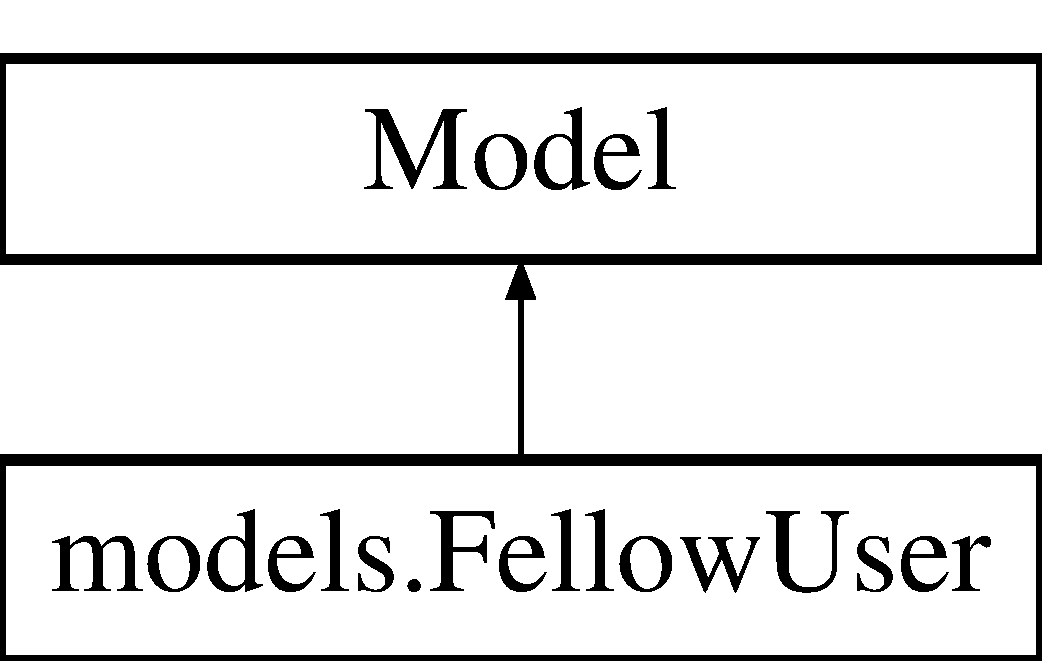
\includegraphics[height=2.000000cm]{classmodels_1_1_fellow_user}
\end{center}
\end{figure}
\subsection*{Public Member Functions}
\begin{DoxyCompactItemize}
\item 
def \hyperlink{classmodels_1_1_fellow_user_ab0b97932b9e3f239b9c65a9878e35381}{\-\_\-\-\_\-unicode\-\_\-\-\_\-}
\begin{DoxyCompactList}\small\item\em Gets model's information in unicode string format. \end{DoxyCompactList}\end{DoxyCompactItemize}
\subsection*{Static Public Attributes}
\begin{DoxyCompactItemize}
\item 
tuple \hyperlink{classmodels_1_1_fellow_user_a5e7120d242fc32956e2b7a0f146d0c86}{user} = models.\-Foreign\-Key(User)
\item 
tuple \hyperlink{classmodels_1_1_fellow_user_aa990390ffe2a4131de17ee9be0afa73b}{owed} = models.\-Decimal\-Field(max\-\_\-digits=11, decimal\-\_\-places=2, default=0)
\end{DoxyCompactItemize}


\subsection{Detailed Description}
Model designed to represent a fellow group member for a single particular \hyperlink{classmodels_1_1_member_view}{Member\-View}. 

\hyperlink{classmodels_1_1_fellow_user}{Fellow\-User} models interact with a \hyperlink{classmodels_1_1_member_view}{Member\-View} model in order to represent the \hyperlink{classmodels_1_1_member_view}{Member\-View}'s balances which they owe their fellow group members. 

\subsection{Member Function Documentation}
\hypertarget{classmodels_1_1_fellow_user_ab0b97932b9e3f239b9c65a9878e35381}{\index{models\-::\-Fellow\-User@{models\-::\-Fellow\-User}!\-\_\-\-\_\-unicode\-\_\-\-\_\-@{\-\_\-\-\_\-unicode\-\_\-\-\_\-}}
\index{\-\_\-\-\_\-unicode\-\_\-\-\_\-@{\-\_\-\-\_\-unicode\-\_\-\-\_\-}!models::FellowUser@{models\-::\-Fellow\-User}}
\subsubsection[{\-\_\-\-\_\-unicode\-\_\-\-\_\-}]{\setlength{\rightskip}{0pt plus 5cm}def models.\-Fellow\-User.\-\_\-\-\_\-unicode\-\_\-\-\_\- (
\begin{DoxyParamCaption}
\item[{}]{self}
\end{DoxyParamCaption}
)}}\label{classmodels_1_1_fellow_user_ab0b97932b9e3f239b9c65a9878e35381}


Gets model's information in unicode string format. 

\begin{DoxyReturn}{Returns}
The fellow user's username 
\end{DoxyReturn}


\subsection{Member Data Documentation}
\hypertarget{classmodels_1_1_fellow_user_aa990390ffe2a4131de17ee9be0afa73b}{\index{models\-::\-Fellow\-User@{models\-::\-Fellow\-User}!owed@{owed}}
\index{owed@{owed}!models::FellowUser@{models\-::\-Fellow\-User}}
\subsubsection[{owed}]{\setlength{\rightskip}{0pt plus 5cm}tuple models.\-Fellow\-User.\-owed = models.\-Decimal\-Field(max\-\_\-digits=11, decimal\-\_\-places=2, default=0)\hspace{0.3cm}{\ttfamily [static]}}}\label{classmodels_1_1_fellow_user_aa990390ffe2a4131de17ee9be0afa73b}
\hypertarget{classmodels_1_1_fellow_user_a5e7120d242fc32956e2b7a0f146d0c86}{\index{models\-::\-Fellow\-User@{models\-::\-Fellow\-User}!user@{user}}
\index{user@{user}!models::FellowUser@{models\-::\-Fellow\-User}}
\subsubsection[{user}]{\setlength{\rightskip}{0pt plus 5cm}tuple models.\-Fellow\-User.\-user = models.\-Foreign\-Key(User)\hspace{0.3cm}{\ttfamily [static]}}}\label{classmodels_1_1_fellow_user_a5e7120d242fc32956e2b7a0f146d0c86}


The documentation for this class was generated from the following file\-:\begin{DoxyCompactItemize}
\item 
\hyperlink{models_8py}{models.\-py}\end{DoxyCompactItemize}

\hypertarget{classforms_1_1_make_group_form}{\section{forms.\-Make\-Group\-Form Class Reference}
\label{classforms_1_1_make_group_form}\index{forms.\-Make\-Group\-Form@{forms.\-Make\-Group\-Form}}
}


A form for creating a new Expen\-Share group.  


Inheritance diagram for forms.\-Make\-Group\-Form\-:\begin{figure}[H]
\begin{center}
\leavevmode
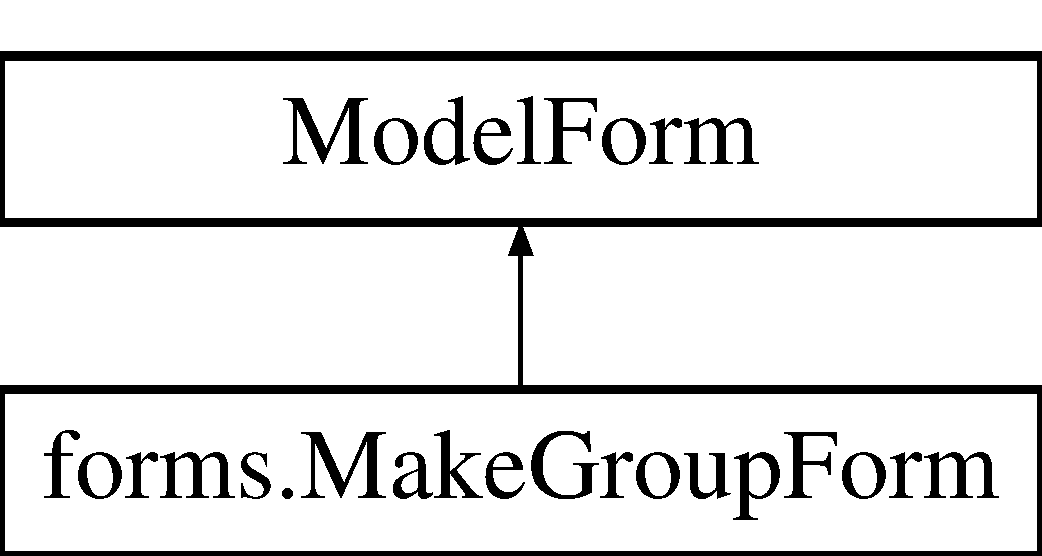
\includegraphics[height=2.000000cm]{classforms_1_1_make_group_form}
\end{center}
\end{figure}
\subsection*{Classes}
\begin{DoxyCompactItemize}
\item 
class \hyperlink{classforms_1_1_make_group_form_1_1_meta}{Meta}
\begin{DoxyCompactList}\small\item\em \hyperlink{classforms_1_1_make_group_form_1_1_meta}{Meta} defines corresponding model (Pay\-Group) and fields. \end{DoxyCompactList}\end{DoxyCompactItemize}
\subsection*{Static Public Attributes}
\begin{DoxyCompactItemize}
\item 
tuple \hyperlink{classforms_1_1_make_group_form_a4d1a913bfafa1caf65dc8b658d94f2e3}{name} = forms.\-Char\-Field(max\-\_\-length=20, label = 'Group Name')
\item 
tuple \hyperlink{classforms_1_1_make_group_form_ad2aa4425d86ae17e396cd0dd26aead15}{description} = forms.\-Char\-Field(max\-\_\-length=50, label = 'Group Description', widget=forms.\-Text\-Input(attrs=\{'size'\-:'37'\}))
\item 
tuple \hyperlink{classforms_1_1_make_group_form_a918fb02b6cb1b6e39e538ee27b42d155}{passcode} = forms.\-Char\-Field(max\-\_\-length=16, label = 'Group Passcode',widget=forms.\-Password\-Input())
\end{DoxyCompactItemize}


\subsection{Detailed Description}
A form for creating a new Expen\-Share group. 

\hyperlink{classforms_1_1_make_group_form}{Make\-Group\-Form} requires a group name, description, and passcode. 

\subsection{Member Data Documentation}
\hypertarget{classforms_1_1_make_group_form_ad2aa4425d86ae17e396cd0dd26aead15}{\index{forms\-::\-Make\-Group\-Form@{forms\-::\-Make\-Group\-Form}!description@{description}}
\index{description@{description}!forms::MakeGroupForm@{forms\-::\-Make\-Group\-Form}}
\subsubsection[{description}]{\setlength{\rightskip}{0pt plus 5cm}tuple forms.\-Make\-Group\-Form.\-description = forms.\-Char\-Field(max\-\_\-length=50, label = 'Group Description', widget=forms.\-Text\-Input(attrs=\{'size'\-:'37'\}))\hspace{0.3cm}{\ttfamily [static]}}}\label{classforms_1_1_make_group_form_ad2aa4425d86ae17e396cd0dd26aead15}
\hypertarget{classforms_1_1_make_group_form_a4d1a913bfafa1caf65dc8b658d94f2e3}{\index{forms\-::\-Make\-Group\-Form@{forms\-::\-Make\-Group\-Form}!name@{name}}
\index{name@{name}!forms::MakeGroupForm@{forms\-::\-Make\-Group\-Form}}
\subsubsection[{name}]{\setlength{\rightskip}{0pt plus 5cm}tuple forms.\-Make\-Group\-Form.\-name = forms.\-Char\-Field(max\-\_\-length=20, label = 'Group Name')\hspace{0.3cm}{\ttfamily [static]}}}\label{classforms_1_1_make_group_form_a4d1a913bfafa1caf65dc8b658d94f2e3}
\hypertarget{classforms_1_1_make_group_form_a918fb02b6cb1b6e39e538ee27b42d155}{\index{forms\-::\-Make\-Group\-Form@{forms\-::\-Make\-Group\-Form}!passcode@{passcode}}
\index{passcode@{passcode}!forms::MakeGroupForm@{forms\-::\-Make\-Group\-Form}}
\subsubsection[{passcode}]{\setlength{\rightskip}{0pt plus 5cm}tuple forms.\-Make\-Group\-Form.\-passcode = forms.\-Char\-Field(max\-\_\-length=16, label = 'Group Passcode',widget=forms.\-Password\-Input())\hspace{0.3cm}{\ttfamily [static]}}}\label{classforms_1_1_make_group_form_a918fb02b6cb1b6e39e538ee27b42d155}


The documentation for this class was generated from the following file\-:\begin{DoxyCompactItemize}
\item 
\hyperlink{forms_8py}{forms.\-py}\end{DoxyCompactItemize}

\hypertarget{classmodels_1_1_member_view}{\section{models.\-Member\-View Class Reference}
\label{classmodels_1_1_member_view}\index{models.\-Member\-View@{models.\-Member\-View}}
}


The \hyperlink{classmodels_1_1_member_view}{Member\-View} model is designed to represent a single group member's view of the expense balances.  


Inheritance diagram for models.\-Member\-View\-:\begin{figure}[H]
\begin{center}
\leavevmode
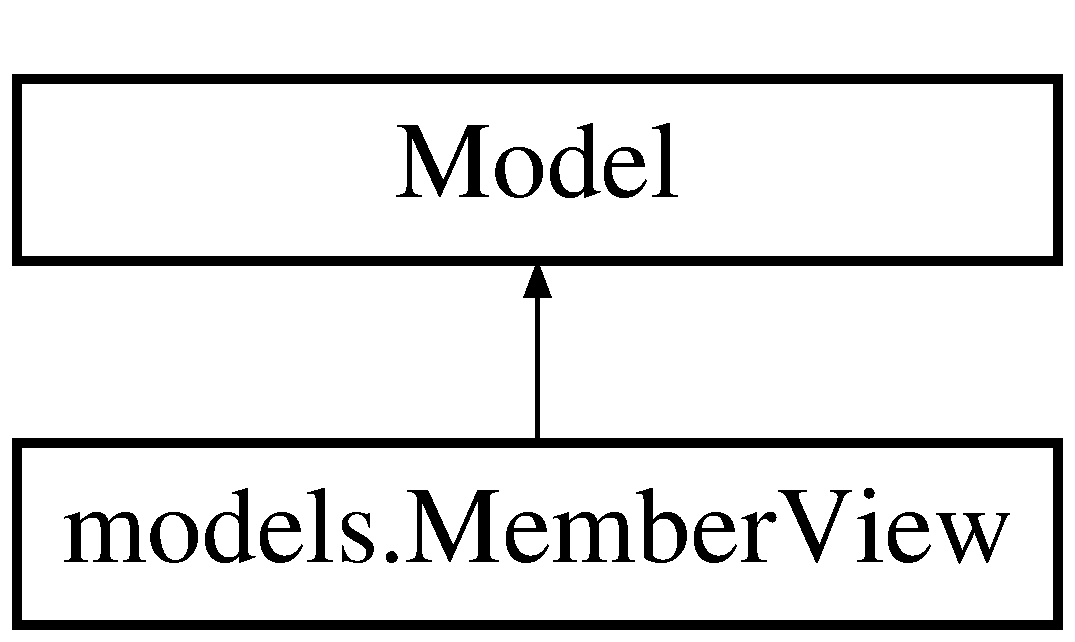
\includegraphics[height=2.000000cm]{classmodels_1_1_member_view}
\end{center}
\end{figure}
\subsection*{Public Member Functions}
\begin{DoxyCompactItemize}
\item 
def \hyperlink{classmodels_1_1_member_view_a362c56c6f6e39dfb3beafd1dd6b9896e}{\-\_\-\-\_\-unicode\-\_\-\-\_\-}
\begin{DoxyCompactList}\small\item\em Gets model's information in unicode string format. \end{DoxyCompactList}\end{DoxyCompactItemize}
\subsection*{Static Public Attributes}
\begin{DoxyCompactItemize}
\item 
tuple \hyperlink{classmodels_1_1_member_view_abb93f3b6aa9cac36c799e0efa49783ff}{user} = models.\-Foreign\-Key(User)
\item 
tuple \hyperlink{classmodels_1_1_member_view_ad008581ab482be3c68ab8b40abfd0fb4}{net\-Owed} = models.\-Decimal\-Field(max\-\_\-digits=11, decimal\-\_\-places=2, default=0)
\item 
tuple \hyperlink{classmodels_1_1_member_view_a021cf8a6e0c3a9fe4d7595fecf7d9d6d}{fellows} = models.\-Many\-To\-Many\-Field(\hyperlink{classmodels_1_1_fellow_user}{Fellow\-User})
\end{DoxyCompactItemize}


\subsection{Detailed Description}
The \hyperlink{classmodels_1_1_member_view}{Member\-View} model is designed to represent a single group member's view of the expense balances. 

\hyperlink{classmodels_1_1_member_view}{Member\-View} represents a particular viewpoint of the expenses. Many Fellow\-Users are associated with a single Memberview. The \hyperlink{classmodels_1_1_member_view}{Member\-View} then represents how much the particular member owes his or her fellow group members. It is a look at the current balance owed to all members from the viewpoint of a particular group member. 

\subsection{Member Function Documentation}
\hypertarget{classmodels_1_1_member_view_a362c56c6f6e39dfb3beafd1dd6b9896e}{\index{models\-::\-Member\-View@{models\-::\-Member\-View}!\-\_\-\-\_\-unicode\-\_\-\-\_\-@{\-\_\-\-\_\-unicode\-\_\-\-\_\-}}
\index{\-\_\-\-\_\-unicode\-\_\-\-\_\-@{\-\_\-\-\_\-unicode\-\_\-\-\_\-}!models::MemberView@{models\-::\-Member\-View}}
\subsubsection[{\-\_\-\-\_\-unicode\-\_\-\-\_\-}]{\setlength{\rightskip}{0pt plus 5cm}def models.\-Member\-View.\-\_\-\-\_\-unicode\-\_\-\-\_\- (
\begin{DoxyParamCaption}
\item[{}]{self}
\end{DoxyParamCaption}
)}}\label{classmodels_1_1_member_view_a362c56c6f6e39dfb3beafd1dd6b9896e}


Gets model's information in unicode string format. 

\begin{DoxyReturn}{Returns}
The member's username 
\end{DoxyReturn}


\subsection{Member Data Documentation}
\hypertarget{classmodels_1_1_member_view_a021cf8a6e0c3a9fe4d7595fecf7d9d6d}{\index{models\-::\-Member\-View@{models\-::\-Member\-View}!fellows@{fellows}}
\index{fellows@{fellows}!models::MemberView@{models\-::\-Member\-View}}
\subsubsection[{fellows}]{\setlength{\rightskip}{0pt plus 5cm}tuple models.\-Member\-View.\-fellows = models.\-Many\-To\-Many\-Field({\bf Fellow\-User})\hspace{0.3cm}{\ttfamily [static]}}}\label{classmodels_1_1_member_view_a021cf8a6e0c3a9fe4d7595fecf7d9d6d}
\hypertarget{classmodels_1_1_member_view_ad008581ab482be3c68ab8b40abfd0fb4}{\index{models\-::\-Member\-View@{models\-::\-Member\-View}!net\-Owed@{net\-Owed}}
\index{net\-Owed@{net\-Owed}!models::MemberView@{models\-::\-Member\-View}}
\subsubsection[{net\-Owed}]{\setlength{\rightskip}{0pt plus 5cm}tuple models.\-Member\-View.\-net\-Owed = models.\-Decimal\-Field(max\-\_\-digits=11, decimal\-\_\-places=2, default=0)\hspace{0.3cm}{\ttfamily [static]}}}\label{classmodels_1_1_member_view_ad008581ab482be3c68ab8b40abfd0fb4}
\hypertarget{classmodels_1_1_member_view_abb93f3b6aa9cac36c799e0efa49783ff}{\index{models\-::\-Member\-View@{models\-::\-Member\-View}!user@{user}}
\index{user@{user}!models::MemberView@{models\-::\-Member\-View}}
\subsubsection[{user}]{\setlength{\rightskip}{0pt plus 5cm}tuple models.\-Member\-View.\-user = models.\-Foreign\-Key(User)\hspace{0.3cm}{\ttfamily [static]}}}\label{classmodels_1_1_member_view_abb93f3b6aa9cac36c799e0efa49783ff}


The documentation for this class was generated from the following file\-:\begin{DoxyCompactItemize}
\item 
\hyperlink{models_8py}{models.\-py}\end{DoxyCompactItemize}

\hypertarget{classforms_1_1_user_form_1_1_meta}{\section{forms.\-User\-Form.\-Meta Class Reference}
\label{classforms_1_1_user_form_1_1_meta}\index{forms.\-User\-Form.\-Meta@{forms.\-User\-Form.\-Meta}}
}


\hyperlink{classforms_1_1_user_form_1_1_meta}{Meta} defines corresponding model (User) and fields.  


\subsection*{Static Public Attributes}
\begin{DoxyCompactItemize}
\item 
\hyperlink{classforms_1_1_user_form_1_1_meta_a23bd9eb69e69089da04ac7bb727f2419}{model} = User
\item 
tuple \hyperlink{classforms_1_1_user_form_1_1_meta_a3e4e28e78acaca06e2540f7fb1145850}{fields} = ('email', 'username', '\hyperlink{classforms_1_1_user_form_af36c6d916f8374e9c6940810af92d95e}{password}')
\end{DoxyCompactItemize}


\subsection{Detailed Description}
\hyperlink{classforms_1_1_user_form_1_1_meta}{Meta} defines corresponding model (User) and fields. 

\subsection{Member Data Documentation}
\hypertarget{classforms_1_1_user_form_1_1_meta_a3e4e28e78acaca06e2540f7fb1145850}{\index{forms\-::\-User\-Form\-::\-Meta@{forms\-::\-User\-Form\-::\-Meta}!fields@{fields}}
\index{fields@{fields}!forms::UserForm::Meta@{forms\-::\-User\-Form\-::\-Meta}}
\subsubsection[{fields}]{\setlength{\rightskip}{0pt plus 5cm}tuple forms.\-User\-Form.\-Meta.\-fields = ('email', 'username', '{\bf password}')\hspace{0.3cm}{\ttfamily [static]}}}\label{classforms_1_1_user_form_1_1_meta_a3e4e28e78acaca06e2540f7fb1145850}
\hypertarget{classforms_1_1_user_form_1_1_meta_a23bd9eb69e69089da04ac7bb727f2419}{\index{forms\-::\-User\-Form\-::\-Meta@{forms\-::\-User\-Form\-::\-Meta}!model@{model}}
\index{model@{model}!forms::UserForm::Meta@{forms\-::\-User\-Form\-::\-Meta}}
\subsubsection[{model}]{\setlength{\rightskip}{0pt plus 5cm}forms.\-User\-Form.\-Meta.\-model = User\hspace{0.3cm}{\ttfamily [static]}}}\label{classforms_1_1_user_form_1_1_meta_a23bd9eb69e69089da04ac7bb727f2419}


The documentation for this class was generated from the following file\-:\begin{DoxyCompactItemize}
\item 
\hyperlink{forms_8py}{forms.\-py}\end{DoxyCompactItemize}

\hypertarget{classforms_1_1_pay_form_1_1_meta}{\section{forms.\-Pay\-Form.\-Meta Class Reference}
\label{classforms_1_1_pay_form_1_1_meta}\index{forms.\-Pay\-Form.\-Meta@{forms.\-Pay\-Form.\-Meta}}
}


\hyperlink{classforms_1_1_pay_form_1_1_meta}{Meta} defines corresponding model (Payment\-Log) and fields.  


\subsection*{Static Public Attributes}
\begin{DoxyCompactItemize}
\item 
\hyperlink{classforms_1_1_pay_form_1_1_meta_a0d19bc0415cefc2cb26290e36ecb16e3}{model} = \hyperlink{classmodels_1_1_payment_log}{models.\-Payment\-Log}
\item 
tuple \hyperlink{classforms_1_1_pay_form_1_1_meta_a60fd0e31aecbc3e3265aa1103edac965}{fields} = ('\hyperlink{classforms_1_1_pay_form_a5d1483bf91d02813dc5e452d98beb013}{amount}', '\hyperlink{classforms_1_1_pay_form_a39a3a28d0b444a5e47b103b7fe36c476}{description}')
\end{DoxyCompactItemize}


\subsection{Detailed Description}
\hyperlink{classforms_1_1_pay_form_1_1_meta}{Meta} defines corresponding model (Payment\-Log) and fields. 

\subsection{Member Data Documentation}
\hypertarget{classforms_1_1_pay_form_1_1_meta_a60fd0e31aecbc3e3265aa1103edac965}{\index{forms\-::\-Pay\-Form\-::\-Meta@{forms\-::\-Pay\-Form\-::\-Meta}!fields@{fields}}
\index{fields@{fields}!forms::PayForm::Meta@{forms\-::\-Pay\-Form\-::\-Meta}}
\subsubsection[{fields}]{\setlength{\rightskip}{0pt plus 5cm}tuple forms.\-Pay\-Form.\-Meta.\-fields = ('{\bf amount}', '{\bf description}')\hspace{0.3cm}{\ttfamily [static]}}}\label{classforms_1_1_pay_form_1_1_meta_a60fd0e31aecbc3e3265aa1103edac965}
\hypertarget{classforms_1_1_pay_form_1_1_meta_a0d19bc0415cefc2cb26290e36ecb16e3}{\index{forms\-::\-Pay\-Form\-::\-Meta@{forms\-::\-Pay\-Form\-::\-Meta}!model@{model}}
\index{model@{model}!forms::PayForm::Meta@{forms\-::\-Pay\-Form\-::\-Meta}}
\subsubsection[{model}]{\setlength{\rightskip}{0pt plus 5cm}forms.\-Pay\-Form.\-Meta.\-model = {\bf models.\-Payment\-Log}\hspace{0.3cm}{\ttfamily [static]}}}\label{classforms_1_1_pay_form_1_1_meta_a0d19bc0415cefc2cb26290e36ecb16e3}


The documentation for this class was generated from the following file\-:\begin{DoxyCompactItemize}
\item 
\hyperlink{forms_8py}{forms.\-py}\end{DoxyCompactItemize}

\hypertarget{classforms_1_1_make_group_form_1_1_meta}{\section{forms.\-Make\-Group\-Form.\-Meta Class Reference}
\label{classforms_1_1_make_group_form_1_1_meta}\index{forms.\-Make\-Group\-Form.\-Meta@{forms.\-Make\-Group\-Form.\-Meta}}
}


\hyperlink{classforms_1_1_make_group_form_1_1_meta}{Meta} defines corresponding model (Pay\-Group) and fields.  


\subsection*{Static Public Attributes}
\begin{DoxyCompactItemize}
\item 
\hyperlink{classforms_1_1_make_group_form_1_1_meta_ac29614b76d655e69c45c88b40a21c16e}{model} = \hyperlink{classmodels_1_1_pay_group}{models.\-Pay\-Group}
\item 
tuple \hyperlink{classforms_1_1_make_group_form_1_1_meta_ae92fd41d182c3c9b6bb23221993839f5}{fields} = ('\hyperlink{classforms_1_1_make_group_form_a4d1a913bfafa1caf65dc8b658d94f2e3}{name}', '\hyperlink{classforms_1_1_make_group_form_ad2aa4425d86ae17e396cd0dd26aead15}{description}', '\hyperlink{classforms_1_1_make_group_form_a918fb02b6cb1b6e39e538ee27b42d155}{passcode}')
\end{DoxyCompactItemize}


\subsection{Detailed Description}
\hyperlink{classforms_1_1_make_group_form_1_1_meta}{Meta} defines corresponding model (Pay\-Group) and fields. 

\subsection{Member Data Documentation}
\hypertarget{classforms_1_1_make_group_form_1_1_meta_ae92fd41d182c3c9b6bb23221993839f5}{\index{forms\-::\-Make\-Group\-Form\-::\-Meta@{forms\-::\-Make\-Group\-Form\-::\-Meta}!fields@{fields}}
\index{fields@{fields}!forms::MakeGroupForm::Meta@{forms\-::\-Make\-Group\-Form\-::\-Meta}}
\subsubsection[{fields}]{\setlength{\rightskip}{0pt plus 5cm}tuple forms.\-Make\-Group\-Form.\-Meta.\-fields = ('{\bf name}', '{\bf description}', '{\bf passcode}')\hspace{0.3cm}{\ttfamily [static]}}}\label{classforms_1_1_make_group_form_1_1_meta_ae92fd41d182c3c9b6bb23221993839f5}
\hypertarget{classforms_1_1_make_group_form_1_1_meta_ac29614b76d655e69c45c88b40a21c16e}{\index{forms\-::\-Make\-Group\-Form\-::\-Meta@{forms\-::\-Make\-Group\-Form\-::\-Meta}!model@{model}}
\index{model@{model}!forms::MakeGroupForm::Meta@{forms\-::\-Make\-Group\-Form\-::\-Meta}}
\subsubsection[{model}]{\setlength{\rightskip}{0pt plus 5cm}forms.\-Make\-Group\-Form.\-Meta.\-model = {\bf models.\-Pay\-Group}\hspace{0.3cm}{\ttfamily [static]}}}\label{classforms_1_1_make_group_form_1_1_meta_ac29614b76d655e69c45c88b40a21c16e}


The documentation for this class was generated from the following file\-:\begin{DoxyCompactItemize}
\item 
\hyperlink{forms_8py}{forms.\-py}\end{DoxyCompactItemize}

\hypertarget{classforms_1_1_pay_form}{\section{forms.\-Pay\-Form Class Reference}
\label{classforms_1_1_pay_form}\index{forms.\-Pay\-Form@{forms.\-Pay\-Form}}
}


A form for entering an expense amount and description.  


Inheritance diagram for forms.\-Pay\-Form\-:\begin{figure}[H]
\begin{center}
\leavevmode
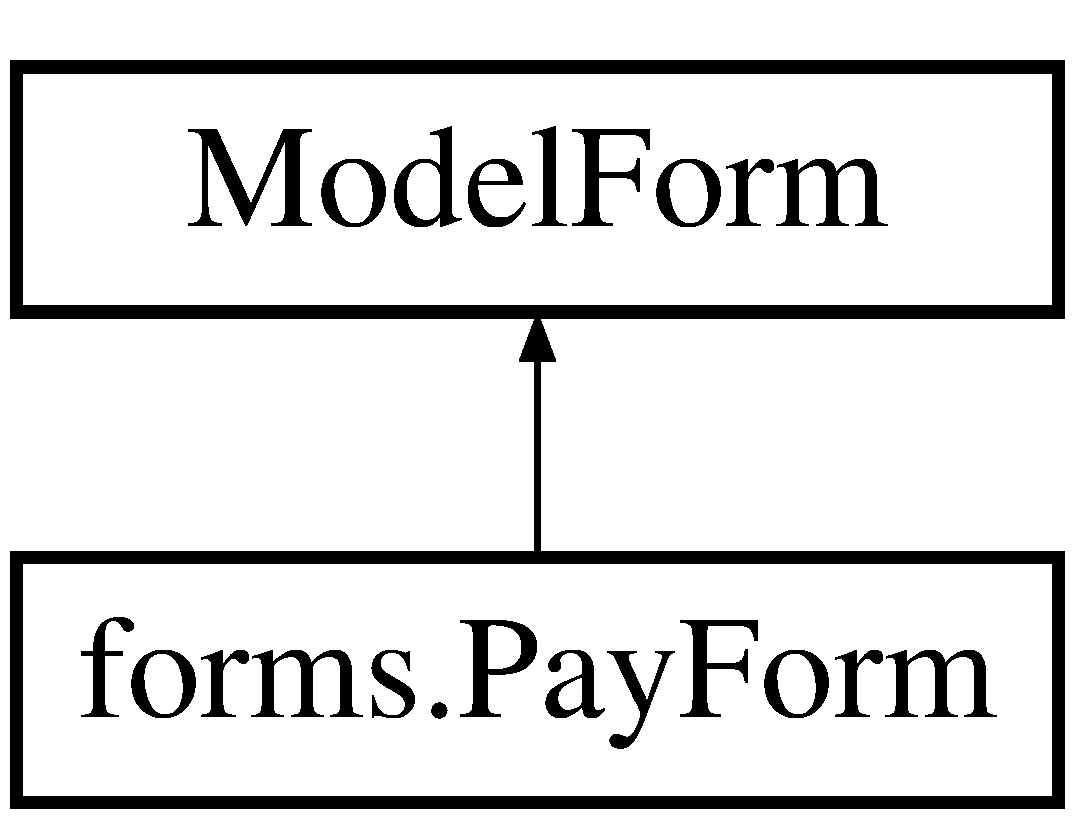
\includegraphics[height=2.000000cm]{classforms_1_1_pay_form}
\end{center}
\end{figure}
\subsection*{Classes}
\begin{DoxyCompactItemize}
\item 
class \hyperlink{classforms_1_1_pay_form_1_1_meta}{Meta}
\begin{DoxyCompactList}\small\item\em \hyperlink{classforms_1_1_pay_form_1_1_meta}{Meta} defines corresponding model (Payment\-Log) and fields. \end{DoxyCompactList}\end{DoxyCompactItemize}
\subsection*{Static Public Attributes}
\begin{DoxyCompactItemize}
\item 
tuple \hyperlink{classforms_1_1_pay_form_a5d1483bf91d02813dc5e452d98beb013}{amount} = forms.\-Decimal\-Field(max\-\_\-digits=11, decimal\-\_\-places=2, label = 'Amount')
\item 
tuple \hyperlink{classforms_1_1_pay_form_a39a3a28d0b444a5e47b103b7fe36c476}{description} = forms.\-Char\-Field(max\-\_\-length=50, label = 'Description')
\end{DoxyCompactItemize}


\subsection{Detailed Description}
A form for entering an expense amount and description. 

\subsection{Member Data Documentation}
\hypertarget{classforms_1_1_pay_form_a5d1483bf91d02813dc5e452d98beb013}{\index{forms\-::\-Pay\-Form@{forms\-::\-Pay\-Form}!amount@{amount}}
\index{amount@{amount}!forms::PayForm@{forms\-::\-Pay\-Form}}
\subsubsection[{amount}]{\setlength{\rightskip}{0pt plus 5cm}tuple forms.\-Pay\-Form.\-amount = forms.\-Decimal\-Field(max\-\_\-digits=11, decimal\-\_\-places=2, label = 'Amount')\hspace{0.3cm}{\ttfamily [static]}}}\label{classforms_1_1_pay_form_a5d1483bf91d02813dc5e452d98beb013}
\hypertarget{classforms_1_1_pay_form_a39a3a28d0b444a5e47b103b7fe36c476}{\index{forms\-::\-Pay\-Form@{forms\-::\-Pay\-Form}!description@{description}}
\index{description@{description}!forms::PayForm@{forms\-::\-Pay\-Form}}
\subsubsection[{description}]{\setlength{\rightskip}{0pt plus 5cm}tuple forms.\-Pay\-Form.\-description = forms.\-Char\-Field(max\-\_\-length=50, label = 'Description')\hspace{0.3cm}{\ttfamily [static]}}}\label{classforms_1_1_pay_form_a39a3a28d0b444a5e47b103b7fe36c476}


The documentation for this class was generated from the following file\-:\begin{DoxyCompactItemize}
\item 
\hyperlink{forms_8py}{forms.\-py}\end{DoxyCompactItemize}

\hypertarget{classmodels_1_1_pay_group}{\section{models.\-Pay\-Group Class Reference}
\label{classmodels_1_1_pay_group}\index{models.\-Pay\-Group@{models.\-Pay\-Group}}
}


Model for an Expen\-Share group.  


Inheritance diagram for models.\-Pay\-Group\-:\begin{figure}[H]
\begin{center}
\leavevmode
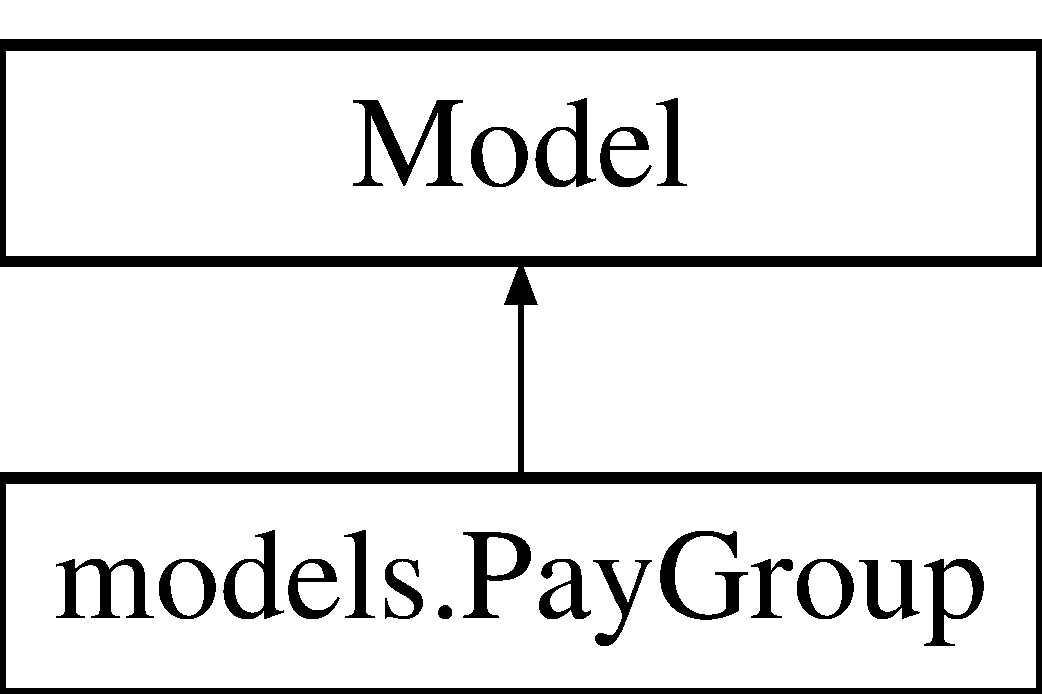
\includegraphics[height=2.000000cm]{classmodels_1_1_pay_group}
\end{center}
\end{figure}
\subsection*{Public Member Functions}
\begin{DoxyCompactItemize}
\item 
def \hyperlink{classmodels_1_1_pay_group_afbeee453535c8f38576fe70759a2e90b}{\-\_\-\-\_\-unicode\-\_\-\-\_\-}
\begin{DoxyCompactList}\small\item\em Gets model's information in unicode string format. \end{DoxyCompactList}\end{DoxyCompactItemize}
\subsection*{Static Public Attributes}
\begin{DoxyCompactItemize}
\item 
tuple \hyperlink{classmodels_1_1_pay_group_a497a5404b56ea78ec8ac675985519c25}{name} = models.\-Char\-Field(max\-\_\-length=20, default=\char`\"{}\char`\"{}, unique=True)
\item 
tuple \hyperlink{classmodels_1_1_pay_group_ae8d4cfe4930ebc6b511f82691026a7d7}{description} = models.\-Char\-Field(max\-\_\-length=50, default=\char`\"{}\char`\"{})
\item 
tuple \hyperlink{classmodels_1_1_pay_group_a22c5aadb801b4f26a4c5f675c628cd64}{members} = models.\-Many\-To\-Many\-Field(User)
\item 
tuple \hyperlink{classmodels_1_1_pay_group_a757bf14853860015be63c29d9f4a4b76}{passcode} = models.\-Char\-Field(max\-\_\-length=16, default=\char`\"{}\char`\"{})
\item 
tuple \hyperlink{classmodels_1_1_pay_group_acbb50cbe600d3e3f492a99b948bf38a8}{payment\-Logs} = models.\-Many\-To\-Many\-Field(\hyperlink{classmodels_1_1_payment_log}{Payment\-Log})
\item 
tuple \hyperlink{classmodels_1_1_pay_group_ae13451dcaaa8c881df92549d1e2a3417}{member\-Views} = models.\-Many\-To\-Many\-Field(\hyperlink{classmodels_1_1_member_view}{Member\-View})
\item 
tuple \hyperlink{classmodels_1_1_pay_group_a2ffd41ff089917ffe7350eeae498c356}{group\-Size} = models.\-Integer\-Field(default=1)
\end{DoxyCompactItemize}


\subsection{Detailed Description}
Model for an Expen\-Share group. 

\hyperlink{classmodels_1_1_pay_group}{Pay\-Group} is a model designed to represent one expense sharing group. It is associated with multiple members and contains a \hyperlink{classmodels_1_1_member_view}{Member\-View} model per member which represents a members particular view point of the expenses incurred. 

\subsection{Member Function Documentation}
\hypertarget{classmodels_1_1_pay_group_afbeee453535c8f38576fe70759a2e90b}{\index{models\-::\-Pay\-Group@{models\-::\-Pay\-Group}!\-\_\-\-\_\-unicode\-\_\-\-\_\-@{\-\_\-\-\_\-unicode\-\_\-\-\_\-}}
\index{\-\_\-\-\_\-unicode\-\_\-\-\_\-@{\-\_\-\-\_\-unicode\-\_\-\-\_\-}!models::PayGroup@{models\-::\-Pay\-Group}}
\subsubsection[{\-\_\-\-\_\-unicode\-\_\-\-\_\-}]{\setlength{\rightskip}{0pt plus 5cm}def models.\-Pay\-Group.\-\_\-\-\_\-unicode\-\_\-\-\_\- (
\begin{DoxyParamCaption}
\item[{}]{self}
\end{DoxyParamCaption}
)}}\label{classmodels_1_1_pay_group_afbeee453535c8f38576fe70759a2e90b}


Gets model's information in unicode string format. 

\begin{DoxyReturn}{Returns}
The name of the paygroup 
\end{DoxyReturn}


\subsection{Member Data Documentation}
\hypertarget{classmodels_1_1_pay_group_ae8d4cfe4930ebc6b511f82691026a7d7}{\index{models\-::\-Pay\-Group@{models\-::\-Pay\-Group}!description@{description}}
\index{description@{description}!models::PayGroup@{models\-::\-Pay\-Group}}
\subsubsection[{description}]{\setlength{\rightskip}{0pt plus 5cm}tuple models.\-Pay\-Group.\-description = models.\-Char\-Field(max\-\_\-length=50, default=\char`\"{}\char`\"{})\hspace{0.3cm}{\ttfamily [static]}}}\label{classmodels_1_1_pay_group_ae8d4cfe4930ebc6b511f82691026a7d7}
\hypertarget{classmodels_1_1_pay_group_a2ffd41ff089917ffe7350eeae498c356}{\index{models\-::\-Pay\-Group@{models\-::\-Pay\-Group}!group\-Size@{group\-Size}}
\index{group\-Size@{group\-Size}!models::PayGroup@{models\-::\-Pay\-Group}}
\subsubsection[{group\-Size}]{\setlength{\rightskip}{0pt plus 5cm}tuple models.\-Pay\-Group.\-group\-Size = models.\-Integer\-Field(default=1)\hspace{0.3cm}{\ttfamily [static]}}}\label{classmodels_1_1_pay_group_a2ffd41ff089917ffe7350eeae498c356}
\hypertarget{classmodels_1_1_pay_group_a22c5aadb801b4f26a4c5f675c628cd64}{\index{models\-::\-Pay\-Group@{models\-::\-Pay\-Group}!members@{members}}
\index{members@{members}!models::PayGroup@{models\-::\-Pay\-Group}}
\subsubsection[{members}]{\setlength{\rightskip}{0pt plus 5cm}tuple models.\-Pay\-Group.\-members = models.\-Many\-To\-Many\-Field(User)\hspace{0.3cm}{\ttfamily [static]}}}\label{classmodels_1_1_pay_group_a22c5aadb801b4f26a4c5f675c628cd64}
\hypertarget{classmodels_1_1_pay_group_ae13451dcaaa8c881df92549d1e2a3417}{\index{models\-::\-Pay\-Group@{models\-::\-Pay\-Group}!member\-Views@{member\-Views}}
\index{member\-Views@{member\-Views}!models::PayGroup@{models\-::\-Pay\-Group}}
\subsubsection[{member\-Views}]{\setlength{\rightskip}{0pt plus 5cm}tuple models.\-Pay\-Group.\-member\-Views = models.\-Many\-To\-Many\-Field({\bf Member\-View})\hspace{0.3cm}{\ttfamily [static]}}}\label{classmodels_1_1_pay_group_ae13451dcaaa8c881df92549d1e2a3417}
\hypertarget{classmodels_1_1_pay_group_a497a5404b56ea78ec8ac675985519c25}{\index{models\-::\-Pay\-Group@{models\-::\-Pay\-Group}!name@{name}}
\index{name@{name}!models::PayGroup@{models\-::\-Pay\-Group}}
\subsubsection[{name}]{\setlength{\rightskip}{0pt plus 5cm}tuple models.\-Pay\-Group.\-name = models.\-Char\-Field(max\-\_\-length=20, default=\char`\"{}\char`\"{}, unique=True)\hspace{0.3cm}{\ttfamily [static]}}}\label{classmodels_1_1_pay_group_a497a5404b56ea78ec8ac675985519c25}
\hypertarget{classmodels_1_1_pay_group_a757bf14853860015be63c29d9f4a4b76}{\index{models\-::\-Pay\-Group@{models\-::\-Pay\-Group}!passcode@{passcode}}
\index{passcode@{passcode}!models::PayGroup@{models\-::\-Pay\-Group}}
\subsubsection[{passcode}]{\setlength{\rightskip}{0pt plus 5cm}tuple models.\-Pay\-Group.\-passcode = models.\-Char\-Field(max\-\_\-length=16, default=\char`\"{}\char`\"{})\hspace{0.3cm}{\ttfamily [static]}}}\label{classmodels_1_1_pay_group_a757bf14853860015be63c29d9f4a4b76}
\hypertarget{classmodels_1_1_pay_group_acbb50cbe600d3e3f492a99b948bf38a8}{\index{models\-::\-Pay\-Group@{models\-::\-Pay\-Group}!payment\-Logs@{payment\-Logs}}
\index{payment\-Logs@{payment\-Logs}!models::PayGroup@{models\-::\-Pay\-Group}}
\subsubsection[{payment\-Logs}]{\setlength{\rightskip}{0pt plus 5cm}tuple models.\-Pay\-Group.\-payment\-Logs = models.\-Many\-To\-Many\-Field({\bf Payment\-Log})\hspace{0.3cm}{\ttfamily [static]}}}\label{classmodels_1_1_pay_group_acbb50cbe600d3e3f492a99b948bf38a8}


The documentation for this class was generated from the following file\-:\begin{DoxyCompactItemize}
\item 
\hyperlink{models_8py}{models.\-py}\end{DoxyCompactItemize}

\hypertarget{classmodels_1_1_payment_log}{\section{models.\-Payment\-Log Class Reference}
\label{classmodels_1_1_payment_log}\index{models.\-Payment\-Log@{models.\-Payment\-Log}}
}


Model designed to represent a transaction.  


Inheritance diagram for models.\-Payment\-Log\-:\begin{figure}[H]
\begin{center}
\leavevmode
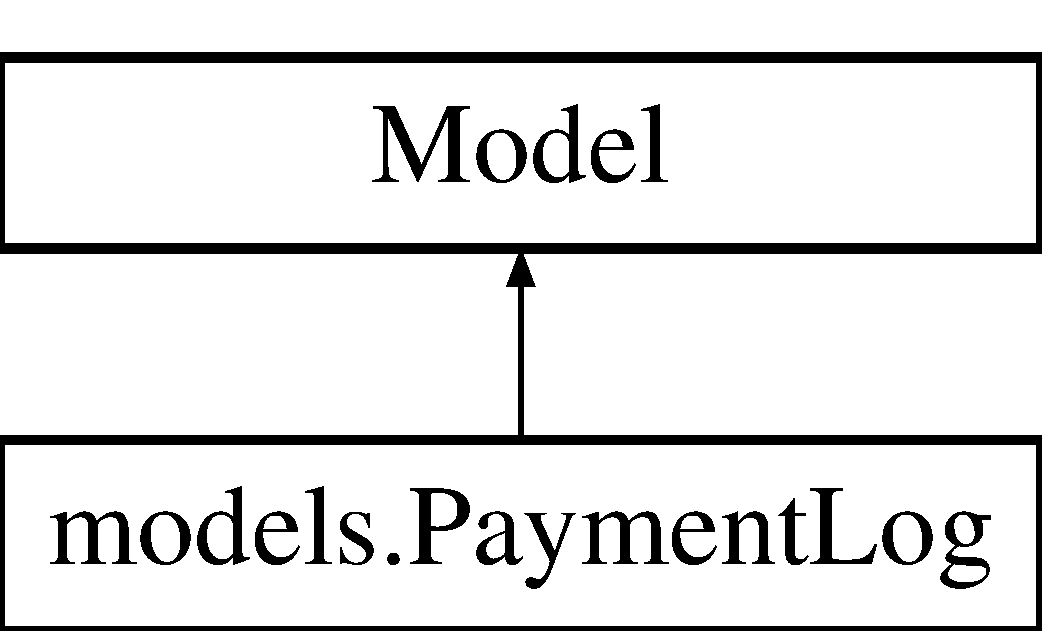
\includegraphics[height=2.000000cm]{classmodels_1_1_payment_log}
\end{center}
\end{figure}
\subsection*{Public Member Functions}
\begin{DoxyCompactItemize}
\item 
def \hyperlink{classmodels_1_1_payment_log_acd2b7422303a0ecade965a291e2a638e}{\-\_\-\-\_\-unicode\-\_\-\-\_\-}
\begin{DoxyCompactList}\small\item\em Gets model's information in unicode string format. \end{DoxyCompactList}\end{DoxyCompactItemize}
\subsection*{Static Public Attributes}
\begin{DoxyCompactItemize}
\item 
tuple \hyperlink{classmodels_1_1_payment_log_a2e40f261b4736e670761066b1de0d081}{amount} = models.\-Decimal\-Field(max\-\_\-digits=11, decimal\-\_\-places=2, default=0)
\item 
tuple \hyperlink{classmodels_1_1_payment_log_ae48129a7de427884354b091e16520e94}{description} = models.\-Char\-Field(max\-\_\-length=50, default=\char`\"{}\char`\"{})
\item 
tuple \hyperlink{classmodels_1_1_payment_log_a52dc6a407079f77462f4be684cf17749}{date} = models.\-Date\-Field(default=time.\-strftime(\char`\"{}\%Y-\/\%m-\/\%d\char`\"{}))
\item 
tuple \hyperlink{classmodels_1_1_payment_log_ac72c158a814c97350349db0a8a091c12}{user} = models.\-Foreign\-Key(User)
\item 
tuple \hyperlink{classmodels_1_1_payment_log_aaeb60280530dfbff5f6f4c17bed6395c}{contested} = models.\-Boolean\-Field(default=False)
\item 
tuple \hyperlink{classmodels_1_1_payment_log_ac1849b45a261444fd1ff697e9e982594}{contested\-Message} = models.\-Char\-Field(max\-\_\-length=140, default=\char`\"{}\char`\"{})
\end{DoxyCompactItemize}


\subsection{Detailed Description}
Model designed to represent a transaction. 

The \hyperlink{classmodels_1_1_payment_log}{Payment\-Log} model is used by a \hyperlink{classmodels_1_1_pay_user}{Pay\-User} when he or she wants to report an Expense. 

\subsection{Member Function Documentation}
\hypertarget{classmodels_1_1_payment_log_acd2b7422303a0ecade965a291e2a638e}{\index{models\-::\-Payment\-Log@{models\-::\-Payment\-Log}!\-\_\-\-\_\-unicode\-\_\-\-\_\-@{\-\_\-\-\_\-unicode\-\_\-\-\_\-}}
\index{\-\_\-\-\_\-unicode\-\_\-\-\_\-@{\-\_\-\-\_\-unicode\-\_\-\-\_\-}!models::PaymentLog@{models\-::\-Payment\-Log}}
\subsubsection[{\-\_\-\-\_\-unicode\-\_\-\-\_\-}]{\setlength{\rightskip}{0pt plus 5cm}def models.\-Payment\-Log.\-\_\-\-\_\-unicode\-\_\-\-\_\- (
\begin{DoxyParamCaption}
\item[{}]{self}
\end{DoxyParamCaption}
)}}\label{classmodels_1_1_payment_log_acd2b7422303a0ecade965a291e2a638e}


Gets model's information in unicode string format. 

\begin{DoxyReturn}{Returns}
Description of the payment log 
\end{DoxyReturn}


\subsection{Member Data Documentation}
\hypertarget{classmodels_1_1_payment_log_a2e40f261b4736e670761066b1de0d081}{\index{models\-::\-Payment\-Log@{models\-::\-Payment\-Log}!amount@{amount}}
\index{amount@{amount}!models::PaymentLog@{models\-::\-Payment\-Log}}
\subsubsection[{amount}]{\setlength{\rightskip}{0pt plus 5cm}tuple models.\-Payment\-Log.\-amount = models.\-Decimal\-Field(max\-\_\-digits=11, decimal\-\_\-places=2, default=0)\hspace{0.3cm}{\ttfamily [static]}}}\label{classmodels_1_1_payment_log_a2e40f261b4736e670761066b1de0d081}
\hypertarget{classmodels_1_1_payment_log_aaeb60280530dfbff5f6f4c17bed6395c}{\index{models\-::\-Payment\-Log@{models\-::\-Payment\-Log}!contested@{contested}}
\index{contested@{contested}!models::PaymentLog@{models\-::\-Payment\-Log}}
\subsubsection[{contested}]{\setlength{\rightskip}{0pt plus 5cm}tuple models.\-Payment\-Log.\-contested = models.\-Boolean\-Field(default=False)\hspace{0.3cm}{\ttfamily [static]}}}\label{classmodels_1_1_payment_log_aaeb60280530dfbff5f6f4c17bed6395c}
\hypertarget{classmodels_1_1_payment_log_ac1849b45a261444fd1ff697e9e982594}{\index{models\-::\-Payment\-Log@{models\-::\-Payment\-Log}!contested\-Message@{contested\-Message}}
\index{contested\-Message@{contested\-Message}!models::PaymentLog@{models\-::\-Payment\-Log}}
\subsubsection[{contested\-Message}]{\setlength{\rightskip}{0pt plus 5cm}tuple models.\-Payment\-Log.\-contested\-Message = models.\-Char\-Field(max\-\_\-length=140, default=\char`\"{}\char`\"{})\hspace{0.3cm}{\ttfamily [static]}}}\label{classmodels_1_1_payment_log_ac1849b45a261444fd1ff697e9e982594}
\hypertarget{classmodels_1_1_payment_log_a52dc6a407079f77462f4be684cf17749}{\index{models\-::\-Payment\-Log@{models\-::\-Payment\-Log}!date@{date}}
\index{date@{date}!models::PaymentLog@{models\-::\-Payment\-Log}}
\subsubsection[{date}]{\setlength{\rightskip}{0pt plus 5cm}tuple models.\-Payment\-Log.\-date = models.\-Date\-Field(default=time.\-strftime(\char`\"{}\%Y-\/\%m-\/\%d\char`\"{}))\hspace{0.3cm}{\ttfamily [static]}}}\label{classmodels_1_1_payment_log_a52dc6a407079f77462f4be684cf17749}
\hypertarget{classmodels_1_1_payment_log_ae48129a7de427884354b091e16520e94}{\index{models\-::\-Payment\-Log@{models\-::\-Payment\-Log}!description@{description}}
\index{description@{description}!models::PaymentLog@{models\-::\-Payment\-Log}}
\subsubsection[{description}]{\setlength{\rightskip}{0pt plus 5cm}tuple models.\-Payment\-Log.\-description = models.\-Char\-Field(max\-\_\-length=50, default=\char`\"{}\char`\"{})\hspace{0.3cm}{\ttfamily [static]}}}\label{classmodels_1_1_payment_log_ae48129a7de427884354b091e16520e94}
\hypertarget{classmodels_1_1_payment_log_ac72c158a814c97350349db0a8a091c12}{\index{models\-::\-Payment\-Log@{models\-::\-Payment\-Log}!user@{user}}
\index{user@{user}!models::PaymentLog@{models\-::\-Payment\-Log}}
\subsubsection[{user}]{\setlength{\rightskip}{0pt plus 5cm}tuple models.\-Payment\-Log.\-user = models.\-Foreign\-Key(User)\hspace{0.3cm}{\ttfamily [static]}}}\label{classmodels_1_1_payment_log_ac72c158a814c97350349db0a8a091c12}


The documentation for this class was generated from the following file\-:\begin{DoxyCompactItemize}
\item 
\hyperlink{models_8py}{models.\-py}\end{DoxyCompactItemize}

\hypertarget{classmodels_1_1_pay_user}{\section{models.\-Pay\-User Class Reference}
\label{classmodels_1_1_pay_user}\index{models.\-Pay\-User@{models.\-Pay\-User}}
}


A model for a user of Expen\-Share.  


Inheritance diagram for models.\-Pay\-User\-:\begin{figure}[H]
\begin{center}
\leavevmode
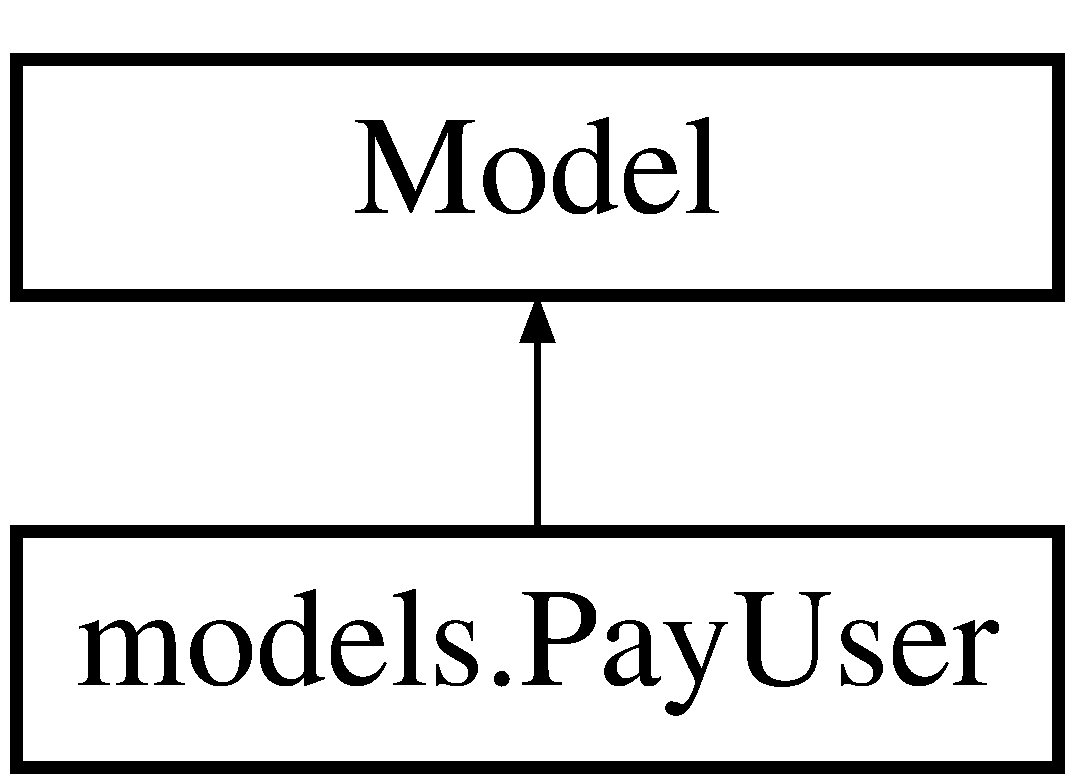
\includegraphics[height=2.000000cm]{classmodels_1_1_pay_user}
\end{center}
\end{figure}
\subsection*{Public Member Functions}
\begin{DoxyCompactItemize}
\item 
def \hyperlink{classmodels_1_1_pay_user_ac491f89a0df97a08ac1f83d1f34e4dfe}{\-\_\-\-\_\-unicode\-\_\-\-\_\-}
\begin{DoxyCompactList}\small\item\em Gets model's information in unicode string format. \end{DoxyCompactList}\end{DoxyCompactItemize}
\subsection*{Static Public Attributes}
\begin{DoxyCompactItemize}
\item 
tuple \hyperlink{classmodels_1_1_pay_user_aa76f651fc85e89f9f366dec5aa0387da}{user\-Key} = models.\-Foreign\-Key(User)
\item 
tuple \hyperlink{classmodels_1_1_pay_user_a719a310f020d573098ebecca7497ba2d}{pay\-Groups} = models.\-Many\-To\-Many\-Field(\hyperlink{classmodels_1_1_pay_group}{Pay\-Group})
\end{DoxyCompactItemize}


\subsection{Detailed Description}
A model for a user of Expen\-Share. 

A \hyperlink{classmodels_1_1_pay_user}{Pay\-User} can join Pay\-Groups and make Payment\-Logs.

A \hyperlink{classmodels_1_1_pay_user}{Pay\-User} corresponds to both a User and a \hyperlink{classmodels_1_1_pay_group}{Pay\-Group} and links them together. 

\subsection{Member Function Documentation}
\hypertarget{classmodels_1_1_pay_user_ac491f89a0df97a08ac1f83d1f34e4dfe}{\index{models\-::\-Pay\-User@{models\-::\-Pay\-User}!\-\_\-\-\_\-unicode\-\_\-\-\_\-@{\-\_\-\-\_\-unicode\-\_\-\-\_\-}}
\index{\-\_\-\-\_\-unicode\-\_\-\-\_\-@{\-\_\-\-\_\-unicode\-\_\-\-\_\-}!models::PayUser@{models\-::\-Pay\-User}}
\subsubsection[{\-\_\-\-\_\-unicode\-\_\-\-\_\-}]{\setlength{\rightskip}{0pt plus 5cm}def models.\-Pay\-User.\-\_\-\-\_\-unicode\-\_\-\-\_\- (
\begin{DoxyParamCaption}
\item[{}]{self}
\end{DoxyParamCaption}
)}}\label{classmodels_1_1_pay_user_ac491f89a0df97a08ac1f83d1f34e4dfe}


Gets model's information in unicode string format. 

\begin{DoxyReturn}{Returns}
The user's key 
\end{DoxyReturn}


\subsection{Member Data Documentation}
\hypertarget{classmodels_1_1_pay_user_a719a310f020d573098ebecca7497ba2d}{\index{models\-::\-Pay\-User@{models\-::\-Pay\-User}!pay\-Groups@{pay\-Groups}}
\index{pay\-Groups@{pay\-Groups}!models::PayUser@{models\-::\-Pay\-User}}
\subsubsection[{pay\-Groups}]{\setlength{\rightskip}{0pt plus 5cm}tuple models.\-Pay\-User.\-pay\-Groups = models.\-Many\-To\-Many\-Field({\bf Pay\-Group})\hspace{0.3cm}{\ttfamily [static]}}}\label{classmodels_1_1_pay_user_a719a310f020d573098ebecca7497ba2d}
\hypertarget{classmodels_1_1_pay_user_aa76f651fc85e89f9f366dec5aa0387da}{\index{models\-::\-Pay\-User@{models\-::\-Pay\-User}!user\-Key@{user\-Key}}
\index{user\-Key@{user\-Key}!models::PayUser@{models\-::\-Pay\-User}}
\subsubsection[{user\-Key}]{\setlength{\rightskip}{0pt plus 5cm}tuple models.\-Pay\-User.\-user\-Key = models.\-Foreign\-Key(User)\hspace{0.3cm}{\ttfamily [static]}}}\label{classmodels_1_1_pay_user_aa76f651fc85e89f9f366dec5aa0387da}


The documentation for this class was generated from the following file\-:\begin{DoxyCompactItemize}
\item 
\hyperlink{models_8py}{models.\-py}\end{DoxyCompactItemize}

\hypertarget{classforms_1_1_user_form}{\section{forms.\-User\-Form Class Reference}
\label{classforms_1_1_user_form}\index{forms.\-User\-Form@{forms.\-User\-Form}}
}


A form for creating a brand new Expen\-Share User.  


Inheritance diagram for forms.\-User\-Form\-:\begin{figure}[H]
\begin{center}
\leavevmode
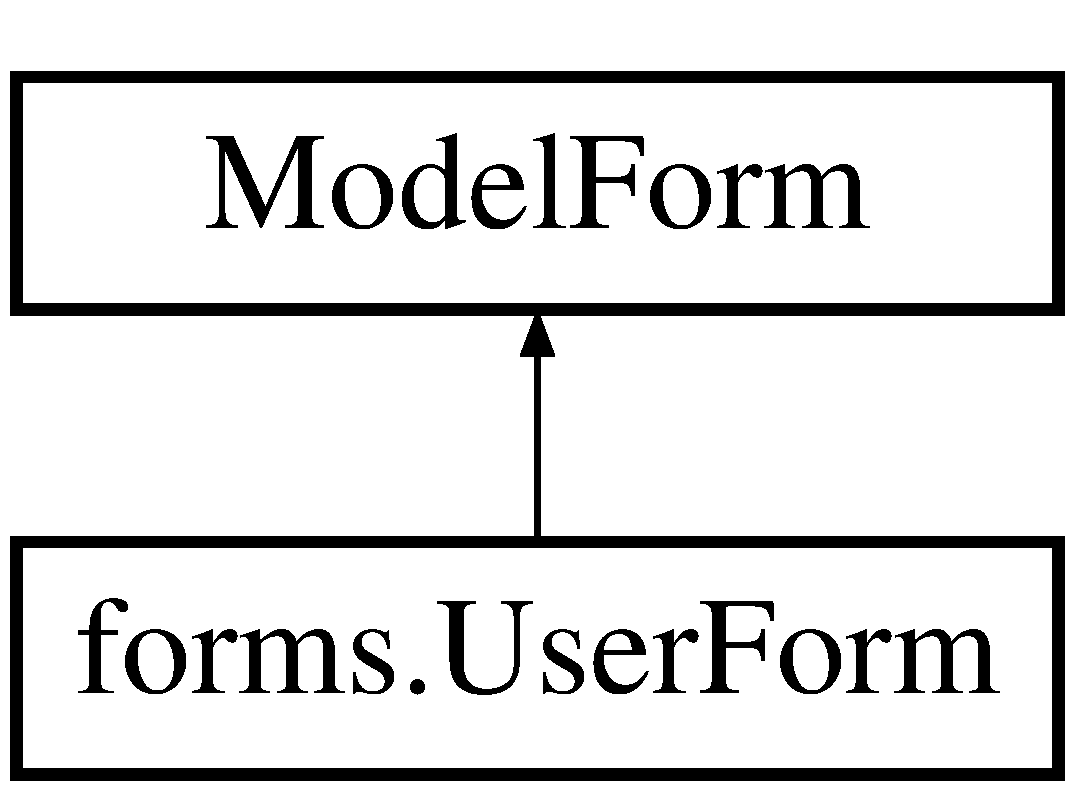
\includegraphics[height=2.000000cm]{classforms_1_1_user_form}
\end{center}
\end{figure}
\subsection*{Classes}
\begin{DoxyCompactItemize}
\item 
class \hyperlink{classforms_1_1_user_form_1_1_meta}{Meta}
\begin{DoxyCompactList}\small\item\em \hyperlink{classforms_1_1_user_form_1_1_meta}{Meta} defines corresponding model (User) and fields. \end{DoxyCompactList}\end{DoxyCompactItemize}
\subsection*{Static Public Attributes}
\begin{DoxyCompactItemize}
\item 
tuple \hyperlink{classforms_1_1_user_form_af36c6d916f8374e9c6940810af92d95e}{password} = forms.\-Char\-Field(widget=forms.\-Password\-Input())
\end{DoxyCompactItemize}


\subsection{Detailed Description}
A form for creating a brand new Expen\-Share User. 

\hyperlink{classforms_1_1_user_form}{User\-Form} requires a password, username, and email. 

\subsection{Member Data Documentation}
\hypertarget{classforms_1_1_user_form_af36c6d916f8374e9c6940810af92d95e}{\index{forms\-::\-User\-Form@{forms\-::\-User\-Form}!password@{password}}
\index{password@{password}!forms::UserForm@{forms\-::\-User\-Form}}
\subsubsection[{password}]{\setlength{\rightskip}{0pt plus 5cm}tuple forms.\-User\-Form.\-password = forms.\-Char\-Field(widget=forms.\-Password\-Input())\hspace{0.3cm}{\ttfamily [static]}}}\label{classforms_1_1_user_form_af36c6d916f8374e9c6940810af92d95e}


The documentation for this class was generated from the following file\-:\begin{DoxyCompactItemize}
\item 
\hyperlink{forms_8py}{forms.\-py}\end{DoxyCompactItemize}

\chapter{File Documentation}
\hypertarget{forms_8py}{\section{forms.\-py File Reference}
\label{forms_8py}\index{forms.\-py@{forms.\-py}}
}


Django forms for taking input from Expen\-Share users.  


\subsection*{Classes}
\begin{DoxyCompactItemize}
\item 
class \hyperlink{classforms_1_1_user_form}{forms.\-User\-Form}
\begin{DoxyCompactList}\small\item\em A form for creating a brand new Expen\-Share User. \end{DoxyCompactList}\item 
class \hyperlink{classforms_1_1_user_form_1_1_meta}{forms.\-User\-Form.\-Meta}
\begin{DoxyCompactList}\small\item\em \hyperlink{classforms_1_1_user_form_1_1_meta}{Meta} defines corresponding model (User) and fields. \end{DoxyCompactList}\item 
class \hyperlink{classforms_1_1_pay_form}{forms.\-Pay\-Form}
\begin{DoxyCompactList}\small\item\em A form for entering an expense amount and description. \end{DoxyCompactList}\item 
class \hyperlink{classforms_1_1_pay_form_1_1_meta}{forms.\-Pay\-Form.\-Meta}
\begin{DoxyCompactList}\small\item\em \hyperlink{classforms_1_1_pay_form_1_1_meta}{Meta} defines corresponding model (Payment\-Log) and fields. \end{DoxyCompactList}\item 
class \hyperlink{classforms_1_1_make_group_form}{forms.\-Make\-Group\-Form}
\begin{DoxyCompactList}\small\item\em A form for creating a new Expen\-Share group. \end{DoxyCompactList}\item 
class \hyperlink{classforms_1_1_make_group_form_1_1_meta}{forms.\-Make\-Group\-Form.\-Meta}
\begin{DoxyCompactList}\small\item\em \hyperlink{classforms_1_1_make_group_form_1_1_meta}{Meta} defines corresponding model (Pay\-Group) and fields. \end{DoxyCompactList}\end{DoxyCompactItemize}
\subsection*{Namespaces}
\begin{DoxyCompactItemize}
\item 
\hyperlink{namespaceforms}{forms}
\end{DoxyCompactItemize}


\subsection{Detailed Description}
Django forms for taking input from Expen\-Share users. \begin{DoxyAuthor}{Authors}
Taylor Andrews, Ian Char, Brennan Mc\-Connell 
\end{DoxyAuthor}
\begin{DoxyDate}{Date}
11/26/2014 
\end{DoxyDate}
\begin{DoxyNote}{Note}
Django Meta class defines non-\/field aspects of django forms. 
\end{DoxyNote}

\hypertarget{mainpage_8dox}{\section{mainpage.\-dox File Reference}
\label{mainpage_8dox}\index{mainpage.\-dox@{mainpage.\-dox}}
}

\hypertarget{models_8py}{\section{models.\-py File Reference}
\label{models_8py}\index{models.\-py@{models.\-py}}
}


Contains the database models implemented by Expen\-Share.  


\subsection*{Classes}
\begin{DoxyCompactItemize}
\item 
class \hyperlink{classmodels_1_1_fellow_user}{models.\-Fellow\-User}
\begin{DoxyCompactList}\small\item\em Model designed to represent a fellow group member for a single particular \hyperlink{classmodels_1_1_member_view}{Member\-View}. \end{DoxyCompactList}\item 
class \hyperlink{classmodels_1_1_member_view}{models.\-Member\-View}
\begin{DoxyCompactList}\small\item\em The \hyperlink{classmodels_1_1_member_view}{Member\-View} model is designed to represent a single group member's view of the expense balances. \end{DoxyCompactList}\item 
class \hyperlink{classmodels_1_1_payment_log}{models.\-Payment\-Log}
\begin{DoxyCompactList}\small\item\em Model designed to represent a transaction. \end{DoxyCompactList}\item 
class \hyperlink{classmodels_1_1_pay_group}{models.\-Pay\-Group}
\begin{DoxyCompactList}\small\item\em Model for an Expen\-Share group. \end{DoxyCompactList}\item 
class \hyperlink{classmodels_1_1_pay_user}{models.\-Pay\-User}
\begin{DoxyCompactList}\small\item\em A model for a user of Expen\-Share. \end{DoxyCompactList}\end{DoxyCompactItemize}
\subsection*{Namespaces}
\begin{DoxyCompactItemize}
\item 
\hyperlink{namespacemodels}{models}
\end{DoxyCompactItemize}


\subsection{Detailed Description}
Contains the database models implemented by Expen\-Share. \begin{DoxyAuthor}{Authors}
Taylor Andrews, Ian Char, Brennan Mc\-Connell 
\end{DoxyAuthor}
\begin{DoxyDate}{Date}
11/26/2014 
\end{DoxyDate}
\begin{DoxyNote}{Note}
The {\bfseries unicode} function allows the models to communicate with Django admin. 
\end{DoxyNote}

\hypertarget{urls_8py}{\section{urls.\-py File Reference}
\label{urls_8py}\index{urls.\-py@{urls.\-py}}
}


U\-R\-L map for Expen\-Share.  


\subsection*{Namespaces}
\begin{DoxyCompactItemize}
\item 
\hyperlink{namespaceurls}{urls}
\end{DoxyCompactItemize}
\subsection*{Variables}
\begin{DoxyCompactItemize}
\item 
tuple \hyperlink{namespaceurls_afac1d3e926b49b028ca292abd72d38a3}{urls.\-urlpatterns}
\begin{DoxyCompactList}\small\item\em Contains all the url tuples for the Expen\-Share website. \end{DoxyCompactList}\end{DoxyCompactItemize}


\subsection{Detailed Description}
U\-R\-L map for Expen\-Share. \begin{DoxyAuthor}{Authors}
Taylor Andrews, Ian Char, Brennan Mc\-Connell 
\end{DoxyAuthor}
\begin{DoxyDate}{Date}
11/25/2014
\end{DoxyDate}
The urlpatterns uses regular expressions to match urls and pass them to views. 
\hypertarget{views_8py}{\section{views.\-py File Reference}
\label{views_8py}\index{views.\-py@{views.\-py}}
}


Contains the functions which implement all the logic behind Expen\-Share.  


\subsection*{Namespaces}
\begin{DoxyCompactItemize}
\item 
\hyperlink{namespaceviews}{views}
\end{DoxyCompactItemize}
\subsection*{Functions}
\begin{DoxyCompactItemize}
\item 
def \hyperlink{namespaceviews_a4902ce68e5b3dd24deea4b61101a31a1}{views.\-index}
\begin{DoxyCompactList}\small\item\em Returns the default Expen\-Share page. \end{DoxyCompactList}\item 
def \hyperlink{namespaceviews_a7e4ef811f9b937ce756922e9eb33812f}{views.\-home}
\begin{DoxyCompactList}\small\item\em Displays the home page for the current User. \end{DoxyCompactList}\item 
def \hyperlink{namespaceviews_a17e3163834c27d86c2907512a2b97ca5}{views.\-history}
\begin{DoxyCompactList}\small\item\em Displays the history webpage which shows all previous expenses for a specific group. \end{DoxyCompactList}\item 
def \hyperlink{namespaceviews_ae6f1a0d94a661eadd45f528456e0f009}{views.\-register}
\begin{DoxyCompactList}\small\item\em This function is used for registering new users. \end{DoxyCompactList}\item 
def \hyperlink{namespaceviews_ae0bc2db6e6831d38b770b4ecc563737e}{views.\-add\-\_\-groupform}
\begin{DoxyCompactList}\small\item\em This function creates a new Pay\-Group. \end{DoxyCompactList}\item 
def \hyperlink{namespaceviews_ae9e7e1e965ecb6fb94b0305f1e353df2}{views.\-add\-\_\-payform}
\begin{DoxyCompactList}\small\item\em Adds an expense to a group. \end{DoxyCompactList}\item 
def \hyperlink{namespaceviews_ac9c9cf0e867f3416d4e954fd6e5d1d77}{views.\-joingroup\-\_\-form}
\begin{DoxyCompactList}\small\item\em Function which allows a User to join an existing Pay\-Group. \end{DoxyCompactList}\item 
def \hyperlink{namespaceviews_a9655dd106f6221c5137d56d511baa503}{views.\-leavegroup}
\begin{DoxyCompactList}\small\item\em Function which makes a user leave a Pay\-Group upon request. \end{DoxyCompactList}\item 
def \hyperlink{namespaceviews_af3df50cbc414500e9838fa25460ad6c1}{views.\-user\-Login}
\begin{DoxyCompactList}\small\item\em Logs a user into their Expen\-Share profile. \end{DoxyCompactList}\item 
def \hyperlink{namespaceviews_af6cfaa4efecee07d037a392fda9ad9cb}{views.\-user\-Logout}
\begin{DoxyCompactList}\small\item\em Logs a User out. \end{DoxyCompactList}\item 
def \hyperlink{namespaceviews_a3e50b5fb508a7d6941b2b8e08a8db21a}{views.\-confirm\-Payment}
\begin{DoxyCompactList}\small\item\em Confirms that a Pay\-User has received payment for existing expenses by a fellow member of the group. \end{DoxyCompactList}\item 
def \hyperlink{namespaceviews_a40ea0e0c6757f628edf4b50461caed99}{views.\-remove\-Pay\-Form}
\begin{DoxyCompactList}\small\item\em Removes a payment from a group. \end{DoxyCompactList}\end{DoxyCompactItemize}


\subsection{Detailed Description}
Contains the functions which implement all the logic behind Expen\-Share. Each view handles various http requests and returns appropriate responses. \begin{DoxyAuthor}{Authors}
Taylor Andrews, Ian Char, Brennan Mc\-Connell 
\end{DoxyAuthor}
\begin{DoxyDate}{Date}
11/26/2014 
\end{DoxyDate}

%--- End generated contents ---

% Index
\newpage
\phantomsection
\addcontentsline{toc}{chapter}{Index}
\printindex

\end{document}
